%%%%%%%%%%%%%%%%%%%%%%%%%%%%%%%%%%%%%%%%%
%  My documentation report
%  Objective: Explain what I did and how, in order to help someone continue with the investigation
%
% Important note:
% Chapter heading images should have a 2:1 width:height ratio,
% e.g. 920px width and 460px height.
%
% The images can be found anywhere, usually on sky surveys websites or the
% Astronomy Picture of the day archive http://apod.nasa.gov/apod/archivepix.html
%
% The original template (the Legrand Orange Book Template) can be found here --> http://www.latextemplates.com/template/the-legrand-orange-book
%
% Original author of the Legrand Orange Book Template:
% Mathias Legrand (legrand.mathias@gmail.com) with modifications by:
% Vel (vel@latextemplates.com)
%
% Original License:
% CC BY-NC-SA 3.0 (http://creativecommons.org/licenses/by-nc-sa/3.0/)
%%%%%%%%%%%%%%%%%%%%%%%%%%%%%%%%%%%%%%%%%
 
%----------------------------------------------------------------------------------------
%	PACKAGES AND OTHER DOCUMENT CONFIGURATIONS
%----------------------------------------------------------------------------------------

\documentclass[11pt,fleqn]{book} % Default font size and left-justified equations

\usepackage[top=3cm,bottom=3cm,left=3.2cm,right=3.2cm,headsep=10pt,letterpaper]{geometry} % Page margins

\usepackage{xcolor} % Required for specifying colors by name
\definecolor{ocre}{RGB}{52,177,201} % Define the orange color used for highlighting throughout the book

% Font Settings
\usepackage{avant} % Use the Avantgarde font for headings
%\usepackage{times} % Use the Times font for headings
\usepackage{mathptmx} % Use the Adobe Times Roman as the default text font together with math symbols from the Sym­bol, Chancery and Com­puter Modern fonts

\usepackage{microtype} % Slightly tweak font spacing for aesthetics
\usepackage[utf8]{inputenc} % Required for including letters with accents
\usepackage[T1]{fontenc} % Use 8-bit encoding that has 256 glyphs

\usepackage{physics} % for physics related notation

% Bibliography
%\usepackage[style=alphabetic,sorting=nyt,sortcites=true,autopunct=true,babel=hyphen,hyperref=true,abbreviate=false,backref=true,backend=biber]{biblatex}
%\addbibresource{bibliography.bib} % BibTeX bibliography file
%\defbibheading{bibempty}{}

%%%%%%%%%%%%%%%%%%%%%%%%%%%%%%%%%%%%%%%%%
% This is based on the Legrand Orange Book
% Structural Definitions File
%
% The original template (the Legrand Orange Book Template) can be found here --> http://www.latextemplates.com/template/the-legrand-orange-book
%
% Original author of the Legrand Orange Book Template::
% Mathias Legrand (legrand.mathias@gmail.com) with modifications by:
% Vel (vel@latextemplates.com)
%
% Original License:
% CC BY-NC-SA 3.0 (http://creativecommons.org/licenses/by-nc-sa/3.0/)
%
%%%%%%%%%%%%%%%%%%%%%%%%%%%%%%%%%%%%%%%%%
%----------------------------------------------------------------------------------------
%	VARIOUS REQUIRED PACKAGES
%----------------------------------------------------------------------------------------

\usepackage{titlesec} % Allows customization of titles

\usepackage{graphicx} % Required for including pictures
\graphicspath{{Pictures/}} % Specifies the directory where pictures are stored

\usepackage{lipsum} % Inserts dummy text

\usepackage{tikz} % Required for drawing custom shapes

\usepackage[english]{babel} % English language/hyphenation

\usepackage{enumitem} % Customize lists
\setlist{nolistsep} % Reduce spacing between bullet points and numbered lists

\usepackage{booktabs} % Required for nicer horizontal rules in tables

\usepackage{eso-pic} % Required for specifying an image background in the title page

%----------------------------------------------------------------------------------------
%	MAIN TABLE OF CONTENTS
%----------------------------------------------------------------------------------------

\usepackage{titletoc} % Required for manipulating the table of contents

\contentsmargin{0cm} % Removes the default margin
% Chapter text styling
\titlecontents{chapter}[1.25cm] % Indentation
{\addvspace{15pt}\large\sffamily\bfseries} % Spacing and font options for chapters
{\color{ocre!60}\contentslabel[\Large\thecontentslabel]{1.25cm}\color{ocre}} % Chapter number
{}  
{\color{ocre!60}\normalsize\sffamily\bfseries\;\titlerule*[.5pc]{.}\;\thecontentspage} % Page number
% Section text styling
\titlecontents{section}[1.25cm] % Indentation
{\addvspace{5pt}\sffamily\bfseries} % Spacing and font options for sections
{\contentslabel[\thecontentslabel]{1.25cm}} % Section number
{}
{\sffamily\hfill\color{black}\thecontentspage} % Page number
[]
% Subsection text styling
\titlecontents{subsection}[1.25cm] % Indentation
{\addvspace{1pt}\sffamily\small} % Spacing and font options for subsections
{\contentslabel[\thecontentslabel]{1.25cm}} % Subsection number
{}
{\sffamily\;\titlerule*[.5pc]{.}\;\thecontentspage} % Page number
[] 

%----------------------------------------------------------------------------------------
%	MINI TABLE OF CONTENTS IN CHAPTER HEADS
%----------------------------------------------------------------------------------------

% Section text styling
\titlecontents{lsection}[0em] % Indendating
{\footnotesize\sffamily} % Font settings
{}
{}
{}

% Subsection text styling
\titlecontents{lsubsection}[.5em] % Indentation
{\normalfont\footnotesize\sffamily} % Font settings
{}
{}
{}
 
%----------------------------------------------------------------------------------------
%	PAGE HEADERS
%----------------------------------------------------------------------------------------

\usepackage{fancyhdr} % Required for header and footer configuration

\pagestyle{fancy}
\renewcommand{\chaptermark}[1]{\markboth{\sffamily\normalsize\bfseries\chaptername\ \thechapter.\ #1}{}} % Chapter text font settings
\renewcommand{\sectionmark}[1]{\markright{\sffamily\normalsize\thesection\hspace{5pt}#1}{}} % Section text font settings
\fancyhf{} \fancyhead[LE,RO]{\sffamily\normalsize\thepage} % Font setting for the page number in the header
\fancyhead[LO]{\rightmark} % Print the nearest section name on the left side of odd pages
\fancyhead[RE]{\leftmark} % Print the current chapter name on the right side of even pages
\renewcommand{\headrulewidth}{0.5pt} % Width of the rule under the header
\addtolength{\headheight}{2.5pt} % Increase the spacing around the header slightly
\renewcommand{\footrulewidth}{0pt} % Removes the rule in the footer
\fancypagestyle{plain}{\fancyhead{}\renewcommand{\headrulewidth}{0pt}} % Style for when a plain pagestyle is specified

% Removes the header from odd empty pages at the end of chapters
\makeatletter
\renewcommand{\cleardoublepage}{
\clearpage\ifodd\c@page\else
\hbox{}
\vspace*{\fill}
\thispagestyle{empty}
\newpage
\fi}

%----------------------------------------------------------------------------------------
%	THEOREM STYLES
%----------------------------------------------------------------------------------------

\usepackage{amsmath,amsfonts,amssymb,amsthm} % For math equations, theorems, symbols, etc

\newcommand{\intoo}[2]{\mathopen{]}#1\,;#2\mathclose{[}}
\newcommand{\ud}{\mathop{\mathrm{{}d}}\mathopen{}}
\newcommand{\intff}[2]{\mathopen{[}#1\,;#2\mathclose{]}}
\newtheorem{notation}{Notation}[chapter]

%%%%%%%%%%%%%%%%%%%%%%%%%%%%%%%%%%%%%%%%%%%%%%%%%%%%%%%%%%%%%%%%%%%%%%%%%%%
%%%%%%%%%%%%%%%%%%%% dedicated to boxed/framed environements %%%%%%%%%%%%%%
%%%%%%%%%%%%%%%%%%%%%%%%%%%%%%%%%%%%%%%%%%%%%%%%%%%%%%%%%%%%%%%%%%%%%%%%%%%
\newtheoremstyle{ocrenumbox}% % Theorem style name
{0pt}% Space above
{0pt}% Space below
{\normalfont}% % Body font
{}% Indent amount
{\small\bf\sffamily\color{ocre}}% % Theorem head font
{\;}% Punctuation after theorem head
{0.25em}% Space after theorem head
{\small\sffamily\color{ocre}\thmname{#1}\nobreakspace\thmnumber{\@ifnotempty{#1}{}\@upn{#2}}% Theorem text (e.g. Theorem 2.1)
\thmnote{\nobreakspace\the\thm@notefont\sffamily\bfseries\color{black}---\nobreakspace#3.}} % Optional theorem note
\renewcommand{\qedsymbol}{$\blacksquare$}% Optional qed square

\newtheoremstyle{blacknumex}% Theorem style name
{5pt}% Space above
{5pt}% Space below
{\normalfont}% Body font
{} % Indent amount
{\small\bf\sffamily}% Theorem head font
{\;}% Punctuation after theorem head
{0.25em}% Space after theorem head
{\small\sffamily{\tiny\ensuremath{\blacksquare}}\nobreakspace\thmname{#1}\nobreakspace\thmnumber{\@ifnotempty{#1}{}\@upn{#2}}% Theorem text (e.g. Theorem 2.1)
\thmnote{\nobreakspace\the\thm@notefont\sffamily\bfseries---\nobreakspace#3.}}% Optional theorem note

\newtheoremstyle{blacknumbox} % Theorem style name
{0pt}% Space above
{0pt}% Space below
{\normalfont}% Body font
{}% Indent amount
{\small\bf\sffamily}% Theorem head font
{\;}% Punctuation after theorem head
{0.25em}% Space after theorem head
{\small\sffamily\thmname{#1}\nobreakspace\thmnumber{\@ifnotempty{#1}{}\@upn{#2}}% Theorem text (e.g. Theorem 2.1)
\thmnote{\nobreakspace\the\thm@notefont\sffamily\bfseries---\nobreakspace#3.}}% Optional theorem note

%%%%%%%%%%%%%%%%%%%%%%%%%%%%%%%%%%%%%%%%%%%%%%%%%%%%%%%%%%%%%%%%%%%%%%%%%%%
%%%%%%%%%%%%% dedicated to non-boxed/non-framed environements %%%%%%%%%%%%%
%%%%%%%%%%%%%%%%%%%%%%%%%%%%%%%%%%%%%%%%%%%%%%%%%%%%%%%%%%%%%%%%%%%%%%%%%%%
\newtheoremstyle{ocrenum}% % Theorem style name
{5pt}% Space above
{5pt}% Space below
{\normalfont}% % Body font
{}% Indent amount
{\small\bf\sffamily\color{ocre}}% % Theorem head font
{\;}% Punctuation after theorem head
{0.25em}% Space after theorem head
{\small\sffamily\color{ocre}\thmname{#1}\nobreakspace\thmnumber{\@ifnotempty{#1}{}\@upn{#2}}% Theorem text (e.g. Theorem 2.1)
\thmnote{\nobreakspace\the\thm@notefont\sffamily\bfseries\color{black}---\nobreakspace#3.}} % Optional theorem note
\renewcommand{\qedsymbol}{$\blacksquare$}% Optional qed square
\makeatother

% Defines the theorem text style for each type of theorem to one of the three styles above
\newcounter{dummy} 
\numberwithin{dummy}{section}
\theoremstyle{ocrenumbox}
\newtheorem{theoremeT}[dummy]{Theorem}
\newtheorem{problem}{Problem}[chapter]
\newtheorem{exerciseT}{Exercise}[chapter]
\theoremstyle{blacknumex}
\newtheorem{exampleT}{Example}[chapter]
\theoremstyle{blacknumbox}
\newtheorem{vocabulary}{Vocabulary}[chapter]
\newtheorem{definitionT}{Definition}[section]
\newtheorem{corollaryT}[dummy]{Corollary}
\theoremstyle{ocrenum}
\newtheorem{proposition}[dummy]{Proposition}

%----------------------------------------------------------------------------------------
%	DEFINITION OF COLORED BOXES
%----------------------------------------------------------------------------------------

\RequirePackage[framemethod=default]{mdframed} % Required for creating the theorem, definition, exercise and corollary boxes

% Theorem box
\newmdenv[skipabove=7pt,
skipbelow=7pt,
backgroundcolor=black!5,
linecolor=ocre,
innerleftmargin=5pt,
innerrightmargin=5pt,
innertopmargin=5pt,
leftmargin=0cm,
rightmargin=0cm,
innerbottommargin=5pt]{tBox}

% Exercise box	  
\newmdenv[skipabove=7pt,
skipbelow=7pt,
rightline=false,
leftline=true,
topline=false,
bottomline=false,
backgroundcolor=ocre!10,
linecolor=ocre,
innerleftmargin=5pt,
innerrightmargin=5pt,
innertopmargin=5pt,
innerbottommargin=5pt,
leftmargin=0cm,
rightmargin=0cm,
linewidth=4pt]{eBox}	

% Definition box
\newmdenv[skipabove=7pt,
skipbelow=7pt,
rightline=false,
leftline=true,
topline=false,
bottomline=false,
linecolor=ocre,
innerleftmargin=5pt,
innerrightmargin=5pt,
innertopmargin=0pt,
leftmargin=0cm,
rightmargin=0cm,
linewidth=4pt,
innerbottommargin=0pt]{dBox}	

% Corollary box
\newmdenv[skipabove=7pt,
skipbelow=7pt,
rightline=false,
leftline=true,
topline=false,
bottomline=false,
linecolor=gray,
backgroundcolor=black!5,
innerleftmargin=5pt,
innerrightmargin=5pt,
innertopmargin=5pt,
leftmargin=0cm,
rightmargin=0cm,
linewidth=4pt,
innerbottommargin=5pt]{cBox}

% Creates an environment for each type of theorem and assigns it a theorem text style from the "Theorem Styles" section above and a colored box from above
\newenvironment{theorem}{\begin{tBox}\begin{theoremeT}}{\end{theoremeT}\end{tBox}}
\newenvironment{exercise}{\begin{eBox}\begin{exerciseT}}{\hfill{\color{ocre}\tiny\ensuremath{\blacksquare}}\end{exerciseT}\end{eBox}}				  
\newenvironment{definition}{\begin{dBox}\begin{definitionT}}{\end{definitionT}\end{dBox}}	
\newenvironment{example}{\begin{exampleT}}{\hfill{\tiny\ensuremath{\blacksquare}}\end{exampleT}}		
\newenvironment{corollary}{\begin{cBox}\begin{corollaryT}}{\end{corollaryT}\end{cBox}}	

%----------------------------------------------------------------------------------------
%	REMARK ENVIRONMENT
%----------------------------------------------------------------------------------------

\newenvironment{remark}{\par\vspace{10pt}\small % Vertical white space above the remark and smaller font size
\begin{list}{}{
\leftmargin=35pt % Indentation on the left
\rightmargin=25pt}\item\ignorespaces % Indentation on the right
\makebox[-2.5pt]{\begin{tikzpicture}[overlay]
\node[draw=ocre!60,line width=1pt,circle,fill=ocre!25,font=\sffamily\bfseries,inner sep=2pt,outer sep=0pt] at (-15pt,0pt){\textcolor{ocre}{R}};\end{tikzpicture}} % Orange R in a circle
\advance\baselineskip -1pt}{\end{list}\vskip5pt} % Tighter line spacing and white space after remark

%----------------------------------------------------------------------------------------
%	SECTION NUMBERING IN THE MARGIN
%----------------------------------------------------------------------------------------

\makeatletter
\renewcommand{\@seccntformat}[1]{\llap{\textcolor{ocre}{\csname the#1\endcsname}\hspace{1em}}}                    
\renewcommand{\section}{\@startsection{section}{1}{\z@}
{-4ex \@plus -1ex \@minus -.4ex}
{1ex \@plus.2ex }
{\normalfont\large\sffamily\bfseries}}
\renewcommand{\subsection}{\@startsection {subsection}{2}{\z@}
{-3ex \@plus -0.1ex \@minus -.4ex}
{0.5ex \@plus.2ex }
{\normalfont\sffamily\bfseries}}
\renewcommand{\subsubsection}{\@startsection {subsubsection}{3}{\z@}
{-2ex \@plus -0.1ex \@minus -.2ex}
{.2ex \@plus.2ex }
{\normalfont\small\sffamily\bfseries}}                        
\renewcommand\paragraph{\@startsection{paragraph}{4}{\z@}
{-2ex \@plus-.2ex \@minus .2ex}
{.1ex}
{\normalfont\small\sffamily\bfseries}}

%----------------------------------------------------------------------------------------
%	HYPERLINKS IN THE DOCUMENTS
%----------------------------------------------------------------------------------------

% For an unclear reason, the package should be loaded now and not later
\usepackage{hyperref}
\hypersetup{hidelinks,backref=true,pagebackref=true,hyperindex=true,colorlinks=false,breaklinks=true,urlcolor= ocre,bookmarks=true,bookmarksopen=false,pdftitle={Title},pdfauthor={Author}}

%----------------------------------------------------------------------------------------
%	CHAPTER HEADINGS
%----------------------------------------------------------------------------------------

% The set-up below should be (sadly) manually adapted to the overall margin page septup controlled by the geometry package loaded in the main.tex document. It is possible to implement below the dimensions used in the goemetry package (top,bottom,left,right)... TO BE DONE

\newcommand{\thechapterimage}{}
\newcommand{\chapterimage}[1]{\renewcommand{\thechapterimage}{#1}}

% Numbered chapters with mini tableofcontents
\def\thechapter{\arabic{chapter}}
\def\@makechapterhead#1{
\thispagestyle{empty}
{\centering \normalfont\sffamily
\ifnum \c@secnumdepth >\m@ne
\if@mainmatter
\startcontents
\begin{tikzpicture}[remember picture,overlay]
\node at (current page.north west)
{\begin{tikzpicture}[remember picture,overlay]
\node[anchor=north west,inner sep=0pt] at (0,0) {\includegraphics[width=\paperwidth]{\thechapterimage}};
%%%%%%%%%%%%%%%%%%%%%%%%%%%%%%%%%%%%%%%%%%%%%%%%%%%%%%%%%%%%%%%%%%%%%%%%%%%%%%%%%%%%%
% Commenting the 3 lines below removes the small contents box in the chapter heading
%\fill[color=ocre!10!white,opacity=.6] (1cm,0) rectangle (8cm,-7cm);
%\node[anchor=north west] at (1.1cm,.35cm) {\parbox[t][8cm][t]{6.5cm}{\huge\bfseries\flushleft \printcontents{l}{1}{\setcounter{tocdepth}{2}}}};
\draw[anchor=west] (5cm,-9cm) node [rounded corners=20pt,fill=ocre!10!white,text opacity=1,draw=ocre,draw opacity=1,line width=1.5pt,fill opacity=.6,inner sep=12pt]{\huge\sffamily\bfseries\textcolor{black}{\thechapter. #1\strut\makebox[22cm]{}}};
%%%%%%%%%%%%%%%%%%%%%%%%%%%%%%%%%%%%%%%%%%%%%%%%%%%%%%%%%%%%%%%%%%%%%%%%%%%%%%%%%%%%%
\end{tikzpicture}};
\end{tikzpicture}}
\par\vspace*{230\p@}
\fi
\fi}

% Unnumbered chapters without mini tableofcontents (could be added though) 
\def\@makeschapterhead#1{
\thispagestyle{empty}
{\centering \normalfont\sffamily
\ifnum \c@secnumdepth >\m@ne
\if@mainmatter
\begin{tikzpicture}[remember picture,overlay]
\node at (current page.north west)
{\begin{tikzpicture}[remember picture,overlay]
\node[anchor=north west,inner sep=0pt] at (0,0) {\includegraphics[width=\paperwidth]{\thechapterimage}};
\draw[anchor=west] (5cm,-9cm) node [rounded corners=20pt,fill=ocre!10!white,fill opacity=.6,inner sep=12pt,text opacity=1,draw=ocre,draw opacity=1,line width=1.5pt]{\huge\sffamily\bfseries\textcolor{black}{#1\strut\makebox[22cm]{}}};
\end{tikzpicture}};
\end{tikzpicture}}
\par\vspace*{230\p@}
\fi
\fi
}
\makeatother % Insert the commands.tex file which contains the majority of the structure behind the template

\begin{document}
\title{Quantum Mechanics}

%----------------------------------------------------------------------------------------
%	TITLE PAGE
%----------------------------------------------------------------------------------------

\begingroup
\thispagestyle{empty}
\AddToShipoutPicture*{\put(0,0){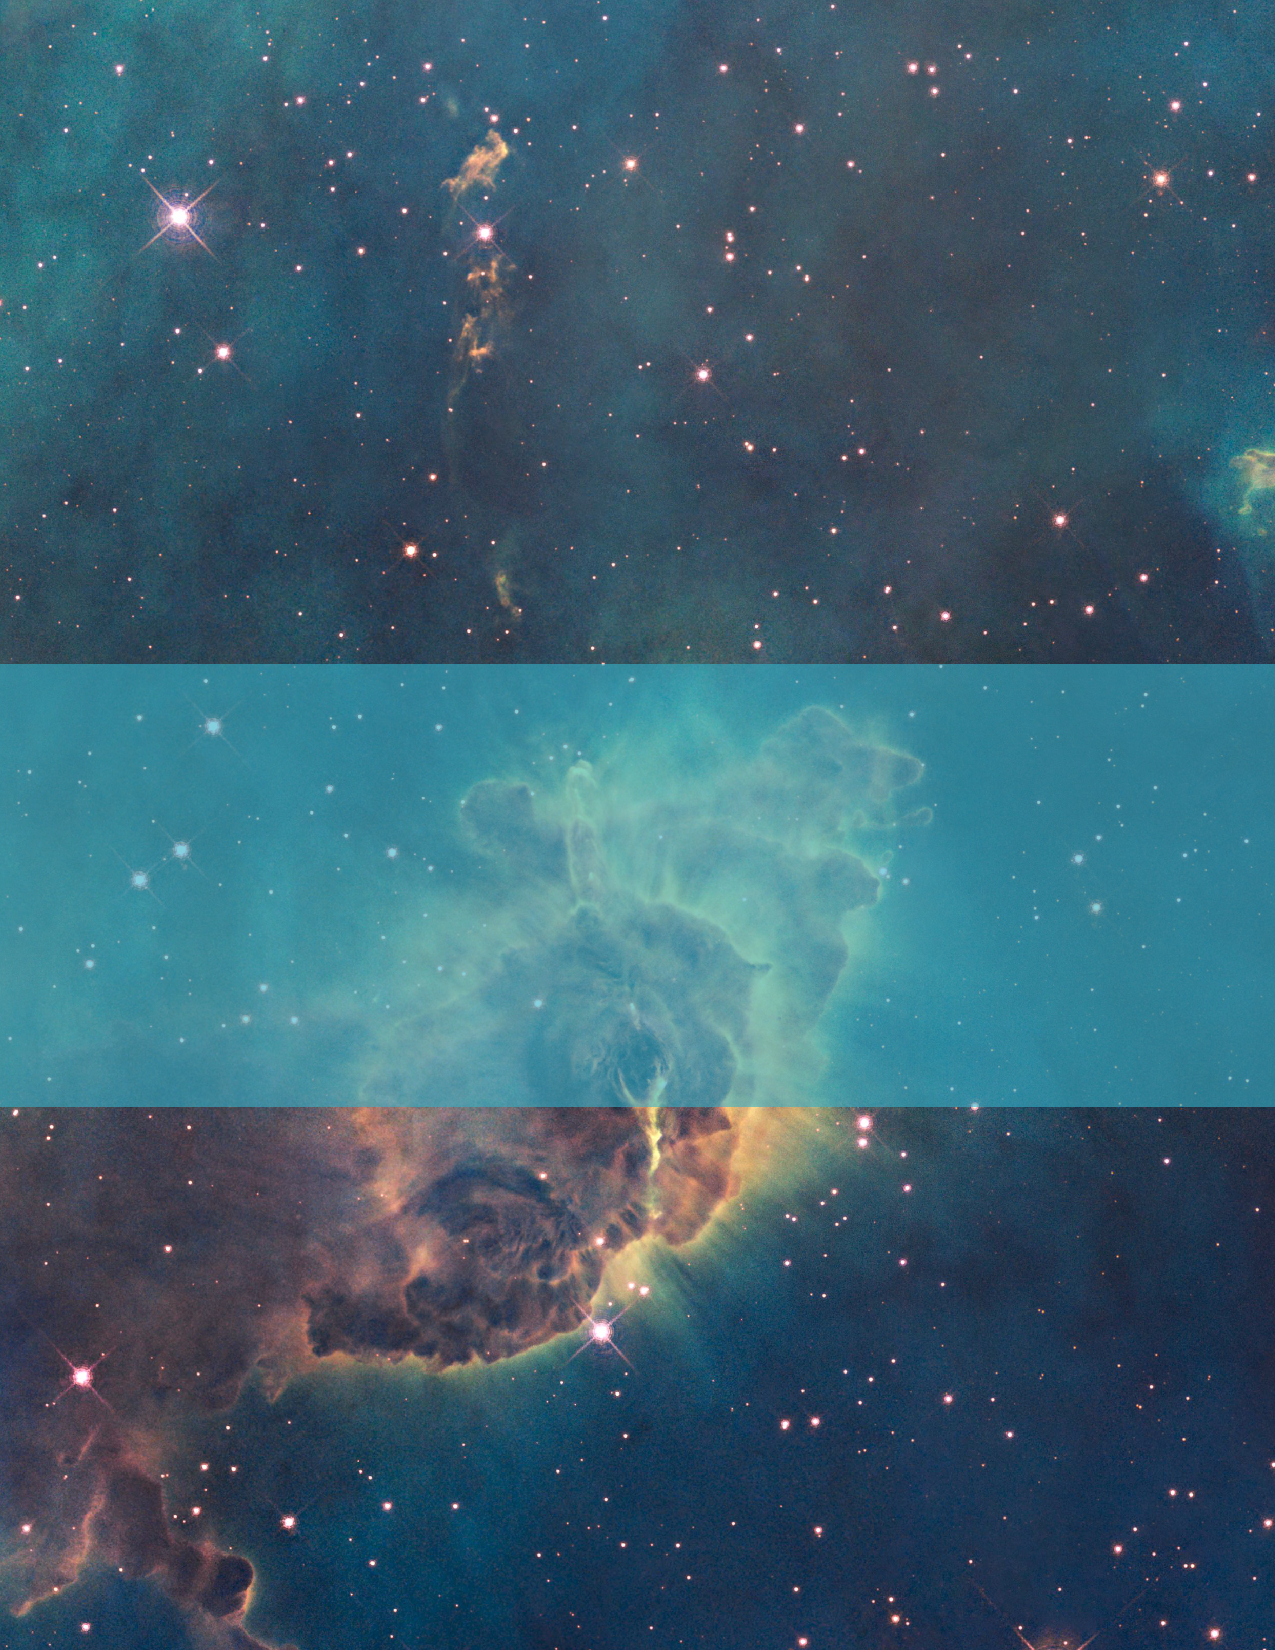
\includegraphics[scale=1.25]{esahubble}}} % Image background
\centering
\vspace*{5cm}
\par\normalfont\fontsize{35}{35}\sffamily\selectfont
\textbf{Quantum Mechanics}\\
{\LARGE Lecture Notes}\par % Book title
\vspace*{1cm}
{\Huge Dr. Khorshed Kabir}\par % Author name
\endgroup

%----------------------------------------------------------------------------------------
%	COPYRIGHT PAGE
%----------------------------------------------------------------------------------------

\newpage
~\vfill
\thispagestyle{empty}

%\noindent Copyright \copyright\ 2014 Andrea Hidalgo\\ % Copyright notice



%\noindent %\textsc{github.com/LaurethTeX/Clustering}\\ % URL

{\noindent This notes are compiled under supervision of Dr. Khorshed Kabir}\\ % License information

{\noindent \textsc{University of Dhaka}}\\

{\noindent \textit{First release, %August
	 2019}} % Printing/edition date

%----------------------------------------------------------------------------------------
%	CREDITS PAGE
%----------------------------------------------------------------------------------------

\newpage


Thanks to the following individuals \\
%\vfill
{\centering
Muhammad Shahnoor Rahman}



%----------------------------------------------------------------------------------------
%	TABLE OF CONTENTS
%----------------------------------------------------------------------------------------

\chapterimage{head1.png} % Table of contents heading image

\pagestyle{empty} % No headers

\tableofcontents % Print the table of contents itself

%\cleardoublepage % Forces the first chapter to start on an odd page so it's on the right

\pagestyle{fancy} % Print headers again
%\pagestyle{headings} % Print headers again

%----------------------------------------------------------------------------------------
%	CHAPTERS
%----------------------------------------------------------------------------------------

\chapterimage{head2.png} % Chapter heading image
\chapter{sheet-1 :Dirac Delta Function}
	Consider the function $D_\epsilon(x)$ given by
	\begin{eqnarray}
	D_\epsilon(x) &= 
		\begin{cases}
			\frac{1}{\epsilon} \ \ &\text{for} \ \  -\frac{\epsilon}{2} \leq x \leq \frac{\epsilon}{2} \\
			0 \ \ &\text{for} \ \  |x| > \frac{\epsilon}{2} 
		\end{cases}
	\end{eqnarray}
	where $\epsilon$ is a positive parameter. The plot of the function is shown below
	
	
	% figure 1
	
	The integral of the function with respect to $x$ is $1$, i.e.,
	\begin{equation}
		\int_{-\infty}^{\infty} D_\epsilon(x) dx = 1
	\end{equation}
	Now imagine making $\epsilon$ smaller. As we decrease $\epsilon$, the function gets narrower and taller, but the integral of the function(i.e., the area under graph remains constant at the value $1$).
	In the limit $\epsilon \rightarrow 0$, the function $D_\epsilon(x)$ collapses to a single  point $x=0$ and gets infinitely tall. So $\lim\limits_{\epsilon \rightarrow \epsilon} D_\epsilon(x)$ is not a function at all and the procedure of taking the limit is not justified.
	\\
	
	However, we can make the limiting procedure meaningful if multiply $D_\epsilon(x)$ by some well defined function $f(x)$, integrate over $x$ and then take the limit $\epsilon \rightarrow 0 $. consider the integral
	\begin{equation}
		\int_{-\infty}^{\infty} D_\epsilon(x) f(x) dx
	\end{equation}
	where $f(x)$ is a well-defined function. If $\epsilon$ is significantly small, the variation of $f(x)$ over the effective integration interval $[-\epsilon / 2, \epsilon / 2]$ is negligible and $f(x)$ remains practically equal to $f(0)$, therefore,
	\begin{equation}
		\int_{-\infty}^{\infty} D_\epsilon (x) f(x) dx \simeq f(0) \int_{-\infty}^{\infty} D_\epsilon (x) dx = f(0)
	\end{equation}
	The smaller the value of $\epsilon$, the better the approximation. In the limit $\epsilon \rightarrow 0$, the above equation is exact
	\begin{equation}
		\lim\limits_{\epsilon \rightarrow 0}\int_{-\infty}^{\infty} D_\epsilon (x) f(x) dx  = f(0)
	\end{equation}
	Now, we define the delta function by the relation
	\begin{equation}
		\int_{-\infty}^{\infty} \delta(x) f(x) dx \  _=^{def}  \lim\limits_{\epsilon \rightarrow 0}\int_{-\infty}^{\infty} D_\epsilon (x) f(x) dx  = f(0)
	\end{equation}
	This equation is valid for any function $f(x)$ defined at the origin. More generally, $\delta(x - x_0)$ is defined as,
	\begin{equation}
		\int_{-\infty}^{\infty} \delta(x - x_0) f(x) dx \ = f(x_0)
	\end{equation}
	Actually, the integral notation $\int_{-\infty}^{\infty} \delta(x) f(x) dx$ is not justified because $\delta(x)$ is not really a function. Physically, there is no problem since it becomes impossible to distinguish between $D_\epsilon(x)$ and $\delta(x)$ as soon as $\epsilon$ becomes negligible compared to all distances involved in a physical problem. Whenever a mathematical difficulty might arise, all we need to do is to assume that $\delta(x)$ is actually $D_\epsilon(x)$ with $\epsilon$ extremely small but not strictly zero.
	\\
	Formally, we can express $\delta(x)$ as a limit of a square of proper functions : 
	\begin{equation}
		\lim\limits_{\epsilon \rightarrow 0} D_\epsilon(x) \equiv \delta(x)
	\end{equation}
	Here $D_\epsilon(x)$, which is a proper function of $x$ is called the representation of the delta function. One representation is the "square function" given at the beginning. The representation is not unique. There are other functions which approach the delta function when appropriate limits are taken.
	
	\section{Other representation of delta function}
		\begin{enumerate}
			\item 
			Consider the function
			\begin{equation}
				D_\epsilon(x) = \frac{1}{\epsilon \sqrt{\pi}} e^{-x^2/\epsilon^2}  \ \ \ (\epsilon > 0)
			\end{equation}
			For each value of the parameter $\epsilon$, this function satisfies
			\begin{equation}
			\int_{-\infty}^{\infty} D_\epsilon(x) dx = 1
			\end{equation}
		
		
		%figure
		
		When plotted against $x$, the function has a peak at the origin. The peak has a height of $\frac{1}{\epsilon \sqrt{\pi}}$ and a width of order $\epsilon$ (exactly how the width is defined doesn't matter). So if $\epsilon$ is allowed to become very small, the peak becomes very tall and very narrow. Outside the peak the function becomes extremely small. Thus we have
		\begin{equation}
		\delta(x) = \lim\limits_{\epsilon \rightarrow 0}\frac{1}{\epsilon \sqrt{\pi}} e^{-x^2/\epsilon^2}
		\end{equation}
		
		%% proof
		
		\item
		Consider another function
		\begin{equation}
			D_\epsilon(x) = \frac{1}{\pi} \frac{\sin(x/\epsilon)}{x} \ \ \ \ (\epsilon > 0)
		\end{equation} 
		
		% figure
		
		For any value of the parameter $\epsilon$ we have 
		\begin{equation}
			\int_{-\infty}^{\infty} D_\epsilon(x) dx = 1
		\end{equation}
		A plot of the function $D_\epsilon(x)$ shows that it has the value $\frac{1}{\epsilon \pi}$ at $x=0$ and it oscillates with decreasing amplitude as $|x|$ increases. The width of the central maxima is of the order of $\epsilon$ and the period of oscillation with respect to $x$ is $2 \pi \epsilon$.\\
		Thus the limit of this function as $\epsilon \rightarrow 0 $ has all the properties of the delta function : it becomes infinitely large at $x=0$, it has unit integral, and infinitely rapid oscillations as $|x|$ increases means that the entire contribution to an integral containing this function comes from an infinitesimal neighborhood of $x=0$.\\
		We can therefore write,
		\begin{equation}
			\delta(x) = \lim\limits_{\epsilon \rightarrow 0} \frac{1}{\pi} \frac{\sin(x/\epsilon)}{x}
		\end{equation}

		\item
		We can also show that
		\begin{eqnarray}
			\delta(x) &= \lim\limits_{\epsilon \rightarrow 0} \frac{1}{2\epsilon} e^{-|x| / \epsilon} \\
			\delta(x) &= \lim\limits_{\epsilon \rightarrow 0} \frac{1}{\pi} \frac{\epsilon}{x^2 + \epsilon^2} \\
			\delta(x) &= \lim\limits_{\epsilon \rightarrow 0} \frac{\epsilon}{\pi} \frac{\sin^2(x/\epsilon)}{x^2}
		\end{eqnarray}
		
		\end{enumerate}	
	\section{Properties of the delta function}
		It is important to note that, because of its singular $@@@@@@$ , the $\delta$ function cannot be the end result of a calculation, and has meaning only so long as a subsequent integral over its argument is carried out. With this understanding we can write down some relations between delta functions.
		\begin{enumerate}[label=\textbf{Property \ \arabic*},start=1]
			\item 
			The delta function is a even function
			\begin{equation}
				\delta(-x) = \delta(x)
			\end{equation}
			
			\item
			\begin{equation}
				x \delta(x) = 0
			\end{equation}
			
			\item
			\begin{equation}
			\delta(a x) = \frac{1}{|a|} \delta(x)
			\end{equation}
			proof: Consider the integral
			\begin{equation}
				I = \int_{-\infty}^{\infty} \delta(a x) f(x) dx
			\end{equation}
			Since the delta function is even in its argument, it doesn't matter if we replace $a$ by $|a|$ in the argument. Thus
			\begin{equation}
				I = \int_{-\infty}^{\infty} \delta(|a| x) f(x) dx
			\end{equation}
			Making the change in variable $ y = |a| x$ we have,
			\begin{eqnarray}
				I &= \frac{1}{|a|}\int_{-\infty}^{\infty} \delta(y) f(y/|a|) dx \nonumber \\
				&= \frac{1}{|a|} f(0) \nonumber
			\end{eqnarray}			
			or
			\begin{equation}
				\int_{-\infty}^{\infty} \delta(a x) f(x) dx = \frac{1}{|a|} \int_{-\infty}^{\infty} \delta(x) f(x) dx
			\end{equation}
			or
			\begin{equation}
				\delta(a x) = \frac{1}{|a|} \delta(x)
			\end{equation}
			
			
			\item
			More generally
			\begin{equation}
				\delta(\phi(x)) = \sum_{i} \frac{\delta(x - x_i)}{\left|\frac{\partial\phi}{\partial x}\right|_{x_i}}
			\end{equation}
			where the sum sums over the $x_i$'s which are simple roots of $\phi(x)$.
			
			proof : let $x_1 , x_2, \ldots , x_N$ be the simple roots of $\phi(x)$,
			
			%figure
			
			In the neighborhood of any one of the simple roots $x_i$, we can write
			\begin{equation}
				\phi(x) = (x - x_i) \psi(x)
			\end{equation}
			where $\psi(x_i) \neq 0$. We have
			\begin{equation}
				\psi(x_i) = \left|\frac{\partial \phi(x)}{\partial x} \right|_{x=x_i}
			\end{equation}
			Now, consider the integral
			\begin{eqnarray}
				I &= \int_{-\infty}^{\infty} \delta(\phi(x)) f(x) dx  \nonumber \\
				&= \sum_{i=1}^{N} \int_{x_i - \epsilon}^{x_i + \epsilon} \delta[(x-x_i) \psi(x_i)] f(x) dx \nonumber \\
				&= \sum_{i=1}^{N} \frac{1}{|\psi(x_i)|}\int_{x_i - \epsilon}^{x_i + \epsilon} \delta(x-x_i) f(x) dx \nonumber \\
				&= \sum_{i=1}^{N} \frac{1}{ \left|\frac{\partial \phi(x)}{\partial x} \right|_{x=x_i}}\int_{-\infty}^{\infty} \delta(x-x_i) f(x) dx \nonumber \\
				&= \sum_{i=1}^{N} \frac{1}{ \left|\frac{\partial \phi}{\partial x} \right|_{x=x_i}} f(x_i) \nonumber
			\end{eqnarray}
			The above result is obtained if we write
			\begin{equation}
				\delta(\phi(x)) = \sum_{i=1}^{N} \frac{\delta(x - x_i)}{\left|\frac{\partial \phi}{\partial x}\right|_{x=x_i}}
			\end{equation}
			
			
			\item
			A frequently used example of the above result is
			\begin{equation}
				\delta(x^2 - a^2) = \frac{1}{2 a} \delta(x - a) + \frac{1}{2 a} \delta(x + a) \ \ \ \ (a > 0)
			\end{equation}
			
			Here
			\begin{equation}
				\phi(x) = x^2 - a^2 = (x-a)(x+a)
			\end{equation}
				The two simple roots of $\phi(x)$ are at $x=a $ and $x=-a$. Now
				\begin{eqnarray}
					\left|\frac{\partial \phi}{\partial x}\right|_{x=a} = \left|2 x\right|_{x=a} = 2a  \\
					\left|\frac{\partial \phi}{\partial x}\right|_{x=a} = \left|-2 x\right|_{x=-a} = 2a 
				\end{eqnarray}
				$\therefore$ The above result follows.
				
				\item
				\begin{equation}
					f(x) \delta(x-a) = f(a) \delta(x-a)
				\end{equation}

				\item
				\begin{equation}
					\int \delta(x-y) \delta(y-a) dy = \delta(x-a)
				\end{equation}
				
			
		\end{enumerate}
		
		\subsection{Notes}
		\begin{enumerate}[label=\textbf{Note : \ \arabic*},start=1]
			\item 
			We have the identity
			\begin{equation}
				x\delta(x) = 0
			\end{equation}
			The converse is also true and it can be shown that the equation
			\begin{equation}
				x u(x) = 0
			\end{equation}
			has the general solution
			\begin{equation}
				u(x) = c \delta(x)
			\end{equation}
			
			
			\item
			We will now prove an identity which is particularly useful in Quantum Mechanics.
			\begin{equation}
				\lim\limits_{\epsilon \rightarrow 0^+} \int_{-\infty}^{\infty} \frac{1}{x \pm \imath \epsilon} f(x) dx = \rho \int_{-\infty}^{\infty} \frac{dx}{x}f(x) \mp \imath\pi f(0)
			\end{equation}
			or in short
			\begin{equation}
				\lim\limits_{\epsilon \rightarrow 0^+} \frac{1}{x \pm \imath \epsilon} = \rho(\frac{1}{x}) \mp \imath \pi \delta(x)
			\end{equation}
			Where it is understood that the second of these two equations have meaning only within an integral.\\
			The symbol $\rho$ means principle part of an integral where the integral has a single pole. The principle part is defined as
			\begin{equation}
				\rho \int_{-A}^{B} \frac{dx}{x} f(x) dx = \lim\limits_{\eta \rightarrow 0^+} \left[\int_{-A}^{-\eta} + \int_{\eta}^{B}\right] \frac{dx}{x} f(x)
			\end{equation}
			\textbf{proof :}
			\begin{equation}
				\frac{1}{x \pm \imath \epsilon} = \frac{x \mp \imath\epsilon}{x^2 + \epsilon^2} = \frac{x}{x^2 + \epsilon^2} \mp \frac{\imath \epsilon}{x^2 + \epsilon^2}
			\end{equation}
			Now we have
			\begin{eqnarray}\label{eqn:1}
				\lim\limits_{\epsilon \rightarrow 0^+} \frac{1}{\pi} \frac{\epsilon}{x^2 + \epsilon^2} &= \delta(x) \nonumber \\
				\lim\limits_{\epsilon \rightarrow 0^+} (\mp) \imath \frac{\epsilon}{x^2 + \epsilon^2} &= \mp \imath \pi \delta(x)
			\end{eqnarray}
			Now consider the first term on the right hand side of equation  \ref{eqn:1}. We multiply this term by a function $f(x)$ which is regular at the origin and then integrate over $x$. We get
			\begin{equation}\label{eqn:2}
				\lim\limits_{\epsilon \rightarrow 0^+} \int_{-\infty}^{\infty} \frac{x f(x)}{x^2 + \epsilon^2} dx
				=\lim\limits_{\epsilon \rightarrow 0^+}\left[
				\lim\limits_{\eta \rightarrow 0^+}\left[ \int_{-\infty}^{-\eta} \frac{x f(x)}{x^2 + \epsilon^2}
				+\int_{-\eta}^{\eta} \frac{x f(x)}{x^2 + \epsilon^2}
				+\int_{\eta}^{\infty} \frac{x f(x)}{x^2 + \epsilon^2} dx\right]\right]
			\end{equation}
			Note that we take the limit over $\eta$ first and then we take the limit over $\epsilon$. Consider now the second integral above
			\begin{equation} 
				\lim\limits_{\eta \rightarrow 0^+} \int_{-\eta}^{+\eta} \frac{x f(x)}{x^2 + \epsilon^2} = f(0) \lim\limits_{\eta \rightarrow 0^+} \frac{1}{2}  \left[\ln({x^2 + \epsilon^2}
				)\right]_{x=-\eta}^{x=\eta} = 0
			\end{equation}
			If we now reverse the order of the evaluation of limits in equation \ref{eqn:2}, the $\epsilon \rightarrow 0$ limit causes no difficulties in the other two integrals.
			Thus we have
			\begin{eqnarray}
				&\lim\limits_{\epsilon \rightarrow 0^+} \int_{-\infty}^{\infty} \frac{x dx}{x^2 + \epsilon^2} f(x)\nonumber \\
				 = &\lim\limits_{\eta \rightarrow 0^+} \lim\limits_{\epsilon \rightarrow 0^+} \left[\int_{-\infty}^{-\eta} + \int_{\eta}^{\infty}\right] \frac{x dx}{x^2 + \epsilon^2} f(x) \nonumber \\
				 = &\lim\limits_{\eta \rightarrow 0^+} \left[\int_{-\infty}^{-\eta} + \int_{\eta}^{\infty}\right] \frac{dx}{x} f(x) \nonumber\\
				 = & \rho \int_{-\infty}^{\infty} \frac{1}{x} f(x) dx \nonumber
			\end{eqnarray}
			This establishes the identity.
		\end{enumerate}
		
	\section{Derivatives of the delta function}
		One may define the derivative $\delta^\prime(x)$ of the delta function. When $\epsilon$ is small, the derivative of $D_\epsilon(x)$ has two peaks close to the origin, one peak is positive and the other is negative as drawn in the figure below
		
		
		% figure
		
		
		As $\epsilon \rightarrow 0$, each of these peaks becomes very narrow and very tall, and two peaks each approach very close to the origin. \\
		Now the integration by parts gives
		\begin{equation}
			\int_{-\infty}^{\infty} dx D_\epsilon^\prime(x) f(x) = \left[D_\epsilon(x) f(x)\right]_{-\infty}^{\infty} - \int_{-\infty}^{\infty} dx D_\epsilon(x) f^\prime(x)
		\end{equation}
		Because $D_\epsilon(x)$ tens to zero as $x \rightarrow \pm \infty$, the first term on the right hand side vanishes unless $f(x)$ $@@@@@@@$ violently at infinity. So by letting $\epsilon \rightarrow 0$, we arrive at the definition of $\delta^\prime(x)$
		\begin{equation}\label{eqn:3}
			\int_{-\infty}^{\infty} \delta^\prime(x) f(x) dx = - \int_{-\infty}^{\infty} \delta(x) f^\prime(x) dx = - f^\prime(0)
		\end{equation}
		From this we immediately get
		\begin{equation}
			x \delta^\prime(x) = -\delta(x)
		\end{equation}
		Conversely, it can be shown that the general solution of the equation
		\begin{equation}
			x u(x) = \delta(x)
		\end{equation}
		can be written as
		\begin{equation}
			u(x) = -\delta^\prime(x) + c \delta(x)
		\end{equation}
		Where the second term arises from the homogeneous equation $x \delta(x) = 0$.
		From equation  \ref{eqn:3}  it also follows that 
		\begin{equation}
			\delta^\prime(-x) = - \delta^\prime(x)
		\end{equation}
		The $n^{th}$ order derivative of $\delta(x)$ can be defined in the same way. We find
		\begin{equation}
			\int_{-\infty}^{\infty} \delta^{(n)}(x) f(x) dx = (-1)^{n} f(0)
		\end{equation}
		We can prove the following properties:
		\begin{eqnarray}
			\delta^{(m)}(x) &= (-1)^m \delta^{(m)} (-x) \\
			x^{m+1} \delta^{(m)}(x) &= 0 \\
			x\delta^{(m)}(x) &= -m \delta^{(m-1)} (x)
		\end{eqnarray}
		
		
	\section{Integration of the delta function}
		Consider the indefinite integral
		\begin{equation}\label{eqn:4}
			\Theta_\epsilon(x) = \int_{-\infty}^{x}  D_\epsilon(y) dy
		\end{equation}
		A graph of $\Theta_\epsilon(x)$ vs $x$ is shown below
		
		%figure
		
		As $\epsilon \rightarrow 0$, the step in the function $\Theta_\epsilon(x)$ gets progressively steeper, until, finally, the function changes abruptly from $0$ to $1$ at $x=0$.
		Thus taking the limit $\epsilon \rightarrow 0$ in equation \ref{eqn:4} we have
		\begin{equation}\label{eqn:5}
			\Theta(x) = \int_{-\infty}^{x} \delta(x) dx
		\end{equation}
		Where
		\begin{equation}
			\Theta(x) = 
			\begin{cases}
				1 \ \ \text{for} \ \ x > 0 \\
				0 \ \ \text{for} \ \ x < 0
			\end{cases}
		\end{equation}
		If we differentiate equation \ref{eqn:5} with respect to $x$,\\
		we get
		\begin{equation}
			\frac{d \Theta(x)}{dx} = \delta(x)
		\end{equation}
		
	\section{Three - dimensional delta function}
		\begin{equation}
			\delta(\vec{r}) _=^{def} \delta(x) \delta(y) \delta(z)
		\end{equation}
		In other words, $\delta(\vec{r})$ is zero if any of the coordinates $x, y, z$ is not equal to zero and $\delta(\vec{r})$ tends to infinity at the origin, i.e., when $x=0, y=0, z=0$, such that 
		\begin{equation}
			\int_{volume} \delta(\vec{r}) d^3 r = 1
		\end{equation}
		if the volume of the integration contains the origin. We also have
		\begin{equation}
			\int \delta(\vec{r}) f(\vec{r}) d^3 r = f(0)
		\end{equation}
		where again the volume of the integration includes the origin.
		\textbf{Note:}
		\begin{eqnarray}
			\delta(\vec{r} - \vec{r^\prime}) &= \delta(x - x^\prime) \delta(y - y^\prime) \delta(z-z^\prime) \\
			\int_{v}\delta(\vec{r} - \vec{r^\prime}) d^3r &= 1
		\end{eqnarray}
		where the volume of integration includes the point $\vec{r}^\prime$. Otherwise the integral is zero.
		\begin{equation}
			\int_{v}\delta(\vec{r} - \vec{r^\prime}) f(\vec{r}) d^3r = f(\vec{r^\prime})
		\end{equation}
		if V includes the point $\vec{r^\prime}$.
		
		\textbf{A useful formula}
		Consider the integral
		\begin{eqnarray}
			\int_{-\infty}^{\infty} e^{\imath k x} dx 
			&= \lim\limits_{L \rightarrow \infty} \int_{-L}^{L} e^{\imath k x} dx \nonumber \\
			&= \lim\limits_{L \rightarrow \infty} \frac{1}{\imath k} \left(e^{\imath k L} - e^{-\imath k L}\right) \nonumber \\
			&= \lim\limits_{L \rightarrow \infty} \frac{2}{k} \left(\frac{e^{\imath k L} - e^{-\imath k L}}{2\imath}\right) \nonumber \\
			&= \lim\limits_{L \rightarrow \infty} \frac{2}{k} \sin(k L) \nonumber \\
			&= 2\pi \lim\limits_{L \rightarrow \infty} \frac{\sin(k L
				)}{\pi k} \nonumber \\
			&= 2\pi \delta(k)
		\end{eqnarray}
		using 
		\begin{equation}
			\lim\limits_{\epsilon \rightarrow 0} \frac{\sin(x /\epsilon
				)}{\pi x} = \delta(x)
		\end{equation}
		Thus
		\begin{equation}\label{eqn:6}
			\int_{-\infty}^{\infty} e^{\imath k x} dx = 2\pi \delta(k)
		\end{equation}
		In equation \ref{eqn:6} if we integrate with respect to $k$, we would have $delta(x)$ on the right hand side,
	
	%%%%%%%%%%%%%%%%%%%%%%%%%%%% equation number
	
		\begin{equation}\label{eqn:100}
		\int_{-\infty}^{\infty} e^{\imath k x} dk = 2\pi \delta(x)
		\end{equation}
		Also note that in equation \ref{eqn:6} we are integrating over its full range of values. Making a change of variable $x \rightarrow -x$ does not change the value of the integral. Hence we also have
		
		\begin{equation}\label{eqn:101}
		\int_{-\infty}^{\infty} e^{-\imath k x} dx = 2\pi \delta(k)
		\end{equation}
		Similarly, in equation \ref{eqn:100} making the change $k \rightarrow -k$, doesn't change the value of the integral. So we could also write
		\begin{equation}\label{eqn:102}
		\int_{-\infty}^{\infty} e^{-\imath k x} dk = 2\pi \delta(x)
		\end{equation}
		
		Thus in summary
		\begin{eqnarray}\label{eqn:103-104}
			\int_{\pm \infty}^{\infty} e^{-\imath k x} dx &= 2\pi \delta(k)
			\int_{\pm \infty}^{\infty} e^{-\imath k x} dk &= 2\pi \delta(x)
		\end{eqnarray}
		In three dimensions
		\begin{eqnarray}\label{eqn:105-107}
			\int_{all\ space} e^{\pm \imath \vec{k} . \vec{r}} d^3\vec{r} &= (2\pi)^3 \delta(\vec{k}) \\
			\int_{all\ space} e^{\pm \imath (\vec{k} - \vec{k^\prime}) . \vec{r}} d^3\vec{r} &= (2\pi)^3 \delta(\vec{k} - \vec{k^\prime}) \\
			\int_{all\ space} e^{\pm \imath \vec{k} . (\vec{r} - \vec{r^\prime})} d^3\vec{r} &= (2\pi)^3 \delta(\vec{r} - \vec{r^\prime}) \\
		\end{eqnarray}
		
	\section{Fourier Transformation}
		We can always express a function $f(x)$ in the form
		\begin{equation}\label{eqn:108}
			f(x) = \int_{-\infty}^{\infty} e^{\imath k x} \tilde{f}(k) dk
		\end{equation}
		where $\tilde{f}(k)$ is a function of $k$, called the fourier transform of $f(x)$. From equation \ref{eqn:108} we can write
		
		\begin{eqnarray}\label{eqn:109}
			\int_{-\infty}^{\infty} e^{-\imath k^\prime x} f(x) dx 
			&= \int_{-\infty}^{\infty} \int_{-\infty}^{\infty} e^{i(k-k^\prime) x} \tilde{f}(k) dk dk^\prime \nonumber \\
			&= 2 \pi \int_{-\infty}^{\infty} \delta(k-k^\prime) \tilde{f}(k) dk \nonumber \\
			&= 2\pi \tilde{f}(k^\prime) 
		\end{eqnarray}
		
		Thus
		\begin{equation}\label{eqn:110}
			\tilde{f}(k) = \frac{1}{2\pi} \int_{-\infty}^{\infty} e^{-\imath k x} f(x) dx
		\end{equation}
		Thus functions $f(x)$ and $\tilde{f}(k)$ are Fourier transform of each other. We can write equation \ref{eqn:108} and \ref{eqn:110} in a more symmetrical fashion as follows:
		\begin{equation}\label{eqn:111}
		f(x) = \frac{1}{\sqrt{2\pi}} \int_{-\infty}^{\infty} e^{\imath k x} \tilde{f}(k) dk
		\end{equation}
		\begin{equation}\label{eqn:112}
			\tilde{f}(k) = \frac{1}{\sqrt{2\pi}} \int_{-\infty}^{\infty} e^{-\imath k x} f(x) dx
		\end{equation}
		In three dimension, we can write
		\begin{equation}\label{eqn:113}
			f(\vec{r}) = \frac{1}{(2\pi)^{3/2}} \int_{all\ k-space} e^{i \vec{k} . \vec{r}} \tilde{f}(\vec{k}) d^3k
		\end{equation}
		multiplying equation \ref{eqn:113} by $e^{-i\vec{k^\prime} . \vec{r}} $ and integrating over $\vec{r}$, we have
		\begin{eqnarray}\label{eqn:114}
			\int_{all\ space} e^{-i\vec{k^\prime} . \vec{r}} f(\vec{r}) d^3 r
			&= \frac{1}{(2\pi)^{3/2}} \int d^3 r \int d^3 k \ e^{i (\vec{k} - \vec{k^\prime}). \vec{r}} \tilde{f}(\vec{k}) \nonumber \\
			&= \frac{1}{(2\pi)^{3/2}} \int d^3 k (2\pi)^3 \delta(\vec{k} - \vec{k^\prime}) \tilde{f}(\vec{k}) \nonumber \\
			&= \frac{1}{(2\pi)^{-3/2}} \tilde{f}(\vec{k^\prime})
		\end{eqnarray}
		
		Therefore
		\begin{equation}\label{eqn:115}
			\tilde{f}(\vec{k}) = \frac{1}{(2\pi)^{3/2}} \int e^{-i\vec{k} . \vec{r}} f(\vec{r}) d^3 r
		\end{equation}
		Thus we can write 
		\begin{equation}\label{eqn:116}
		f(\vec{r}) = \frac{1}{(2\pi)^{3/2}} \int e^{i\vec{k} . \vec{r}} \tilde{f}(\vec{k}) d^3 k
		\end{equation}
		\begin{equation}\label{eqn:117}
		\tilde{f}(\vec{k}) = \frac{1}{(2\pi)^{3/2}} \int e^{-i\vec{k} . \vec{r}} f(\vec{r}) d^3 r
		\end{equation}
		
		\textbf{Parseval's Identity:}\\
		We can now  prove the important identity
		\begin{equation}\label{eqn:118}
			\int |f(\vec{r})|^2 d^3r = \int |\tilde{f}(\vec{k})|^2 d^3k
		\end{equation}
		proof:
		\begin{eqnarray}
			\int |f(\vec{r})|^2 d^3r
			&= \int f(\vec{r}) f^*(\vec{r}) d^3r \nonumber \\
			&= \int d^3r \frac{1}{(2\pi)^{3/2}} \int e^{\imath\vec{k} . \vec{r}} \tilde{f}(\vec{k}) d^3k \frac{1}{(2\pi)^{3/2}} \int e^{-\imath\vec{k^\prime} . \vec{r}} \tilde{f}^*(\vec{k^\prime}) d^3k^\prime \nonumber \\
			&= \frac{1}{(2\pi)^3} \int d^3k\ d^3k^\prime \tilde{f}(\vec{k}) \tilde{f}^*(\vec{k^\prime}) \int d^3r \ e^{\imath(\vec{k} - \vec{k^\prime}).\vec{r}} \nonumber \\
			&= \frac{1}{(2\pi)^3} \int d^3k\ d^3k^\prime \tilde{f}(\vec{k}) \tilde{f}^*(\vec{k^\prime}) (2\pi)^3 \delta(\vec{k} - \vec{k^\prime}) \nonumber \\
			&= \int d^3k\ \tilde{f}(\vec{k}) \tilde{f}^*(\vec{k}) \nonumber \\
			&= \int |\tilde{f}(\vec{k})|^2 d^3k
		\end{eqnarray}
		
		
		
		
		
\chapter{sheet-2 : Linear Vector Space}
References
\begin{enumerate}
	\item 
	Quantum Mechanics	-	Shanker
	
	\item
	Quantum Mechanics	- Sakurai
\end{enumerate}

\section{Definition}
A linear vector space $V$ is a collection of objects $\psi_a, \psi_b, \ldots$, called vectors, which satisfy the following postulates:
\begin{enumerate}
	\item 
	If $\psi_a$ and $\psi_b$ are vectors in $V$, there is a unique vector $\psi_a + \psi_b$ in $V$, called the sum of $\psi_a $ and $\psi_b$. In other words, and operation called addition is defined in the vector space such that the space is closed under addition.
	
	\item 
	The vector addition is commutative and associative, i.e.,
	\begin{eqnarray}\label{eqn:2.1-2.2}
		\psi_a + \psi_b &= \psi_b + \psi_a \\
		\psi_a + (\psi_b + \psi_c) &= (\psi_a + \psi_b) + \psi_c
	\end{eqnarray}
	
	\item 
	There is a vector in $V$ called the null vector and denoted by $\phi$ satisfying
	\begin{equation}\label{eqn:2.3}
	\psi_a + \phi = \phi + \psi_a
	\end{equation}
	for every $\psi_a$ in $V$.
	
	\item 
	For every vector $\psi_a$ in $V$ there is another vector $\psi_a^\prime$ in $V$ such that
	\begin{equation}\label{eqn:2.4}
	\psi_a + \psi_a^\prime = \phi
	\end{equation}
	we denote $\psi_a^\prime$ as $-\psi_a$.\\
	(Note : we use the notation $\psi_a - \psi_b$ to mean $\psi_a + (-\psi_b$).
	
	\item 
	If $\psi_a$ is a vector and $\lambda$ is an arbitrary number (real or complex), called a scaler, there is a uniquely defined vector $\lambda \psi_a$ in $V$ satisfying.
	\begin{enumerate}
		\item 
		\begin{equation}\label{eqn:2.5}
		\lambda (\psi_a  + \psi_b) = \lambda \psi_a + \lambda + \psi_b
		\end{equation}
		i.e., multiplication is distributive with respect to vector addition.
		
		\item 
		\begin{equation}\label{eqn:2.6}
		(\lambda \mu) \psi_a = \lambda (\mu \psi_a)
		\end{equation}
		i.e., multiplication  by a scalar is associative.
		
		\item 
		\begin{equation}\label{eqn:2.7}
		(\lambda + \mu) \psi_a = \lambda \psi_a + \mu \psi_b
		\end{equation}
		i.e., multiplication is distributive with respect to addition scalars.
		
		\item 
		Multiplication by scalars $0$ and $1$ are defined by
		\begin{eqnarray}\label{eqn:2.8-2.9}
			0 \psi_a = \phi \\
			1 \psi_a = \psi_a
		\end{eqnarray}
		for any $\psi_a$ in $V$.
	\end{enumerate}
\end{enumerate}
\section{Example of linear vector space}
\begin{enumerate}
	\item 
	Consider all real numbers $x$ in the range $-\infty$ to $\infty$, i.e.,
	\begin{eqnarray}\label{eqn:2.10-2.11}
		-\infty < x < \infty \\
		x \in \Re \ \ \text{ ($\Re$ is the set of all real numbers )}
	\end{eqnarray}
	Take any two real numbers $x_1$ and $x_2$. If we add two real numbers we get another real number in $\Re$. Thus
	\begin{equation}\label{eqn:2.12}
	x_1 + x_2 = \Re
	\end{equation}
	Next take any real number $x$. If we multiply $x$ by another real number $\lambda$, we get a real number in $\Re$, i.e.,
	\begin{equation}\label{eqn:2.13}
	\lambda x \in \Re
	\end{equation}
	If we take a real number $x$, then there exists another real number $-x$ such that
	\begin{equation}\label{eqn:2.14}
	x + (-x) = 0
	\end{equation}
	So the real numbers form a vector space with the real numbers themselves as vectors in the space. The number $0$ is the null vector $\phi$ of the  space. The scalars $\lambda$ by which the vectors are multiplied are also real numbers.\\
	Thus the real numbers form a real linear vector space over a field which are also real numbers. The addition and multiplication are just the normal addition and multiplication of the real numbers.
	
	\item 
	The set of $n-tuples$ of numbers $(x_1, x_2, \ldots, x_n)$.
	When the addition of vectors and multiplication by a scalar are defined by
	\begin{equation}\label{eqn:2.15}
	(x_1 , x_2, \ldots, x_n) + (y_1 , y_2, \ldots, y_n) = (x_1 + y_1, x_2 + y_2, \ldots, x_n + y_n)
	\end{equation}
	and 
	\begin{equation}\label{eqn:2.16}
	\lambda (x_1, x_2, \ldots, x_n) = (\lambda x_1, \lambda x_2, \ldots, \lambda x_n)
	\end{equation}
	
	
	\item 
	The collection of all square-integrable complex valued functions of a real variable form a vector space. consider all functions
	\begin{equation}\label{eqn:2.17}
	f:\Re \rightarrow \mathbb{C}
	\end{equation}
	here, 
	$\Re $ =  set of real numbers \\
	$\mathbb{C}$  = set of complex numbers\\
	such that
	\begin{equation}\label{eqn:2.18}
	\int_{-\infty}^{\infty} f^*(x) f(x) dx \equiv \int_{-\infty}^{\infty} |f(x)|^2 dx < \infty \text{\  \ (i.e., finite)}
	\end{equation}
	The sum of two functions and the product of a function by a complex scalar are defined in the usual way.\\
	The reason the square-integrable functions form a (complex) vector space is that the space is closed under addition. The vectors of the space are the square-integrable functions. In other words, it can be shown that if $f$ and $g$ are two vectors, in this case two functions $f(x)$ and $g(x)$ both of which are square integrable, then $f(x) + g(x)$ is also square integrable and have the sum belong to the vector space.\\
	\textbf{proof:} \\
	Let $f(x)$ and $g(x)$ be two square integrable function, i.e., 
	\begin{equation}\label{eqn:2.19}
	\int_{-\infty}^{\infty} |f(x)|^2 dx < \infty
	\end{equation}
	and
	\begin{equation}\label{eqn:2.20}
	\int_{-\infty}^{\infty} |g(x)|^2 dx < \infty
	\end{equation}
	then using the inequality
	\begin{equation}\label{eqn:2.21}
	\int_{-\infty}^{\infty} |f+g|^2 dx \leq \left[\sqrt{\int_{\infty}^{\infty} |f|^2 dx} \sqrt{\int_{\infty}^{\infty} |g|^2 dx}\right]^2
	\end{equation}
	it is obvious that
	\begin{equation}\label{eqn:2.22}
	\int_{-\infty}^{\infty} |f+g|^2 dx < \infty
	\end{equation}
	(i.e., finite).
	
	\item 
	The set of all $n\times n$ matrices with complex elements form a complex linear vector space. For illustation let us take $2\times 2$ matrix $A$
	\begin{equation}\label{eqn:2.23}
	A = \left(			
	\begin{matrix}
	a & b \\
	c & d
	\end{matrix}
	\right)
	\end{equation}
	where the elements $a, b, c$ and $d$ can, in general, be complex. Then $A$ belongs to a vector (complex) space.
	We have
	
	\begin{eqnarray}\label{eqn:2.24-2.27}
		\phi &= \left(
		\begin{matrix}
			0 & 0 \\ 0 & 0
		\end{matrix}
		\right)\\
		\mathbb{I} &= \left(
		\begin{matrix}
			1 & 0 \\ 0 & 1
		\end{matrix}
		\right)\\
		-A &= \left(
		\begin{matrix}
			-a & -b \\ -c & -d
		\end{matrix}
		\right)\\
		\lambda A &= \left(
		\begin{matrix}
			\lambda a & \lambda b \\ \lambda c & \lambda d
		\end{matrix}
		\right)
	\end{eqnarray}
	The set of all these matrices form a vector space.						
\end{enumerate}

\section{Inner product space or a unitary vector space}\label{inner_product}
For a general linear vector space, product of vectors (i.e. multiplication of two vectors) need ot be defined. However, we will restrict ourselves to spaces in which a  scalar product or an inner product is defined.\\
A linear vector space is called unitary if a scalar product is defined in it. To every pair of vectors $\psi_a$ and $\psi_b$ in $V$ there corresponds a unique scalar (in general complex), called the scalar product. The scalar product is defined to have the following properties :
\begin{eqnarray}\label{eqn:2.28-2.32}
	(\psi_a , \psi_b) &= (\psi_b, \psi_a)^* \\
	(\psi_a , \lambda \psi_b) &= \lambda (\psi_a , \psi_b) \\
	(\lambda \psi_a , \psi_b) &= \lambda^* (\psi_a , \psi_b) \\
	(\psi_a , \psi_b + \psi_c) &= (\psi_a , \psi_b) + (\psi_a , \psi_c) \\
	(psi_a, \psi_a) \geq 0 \ \text{;the equality holds only if $\psi_a$ is the null vector}
\end{eqnarray}
It follows from the above postulated properties of the scalar product, that the scalar product is linear with respect to post factors, i.e.,
\begin{equation}\label{eqn:2.33}
(\psi_a, \lambda \psi_b + \mu \psi_c) = \lambda (\psi_a , \psi_b) + \mu (\psi_a , \psi_c)
\end{equation}
and anti-linear with respect to the pre factors, i.e.,
\begin{equation}\label{eqn:2.34}
(\lambda \psi_a + \mu \psi_b, \psi_c ) = \lambda^* (\psi_a , \psi_c) + \mu^* (\psi_b , \psi_c)
\end{equation}

\section{Examples of scalar product}
\begin{enumerate}[label=\textbf{Example \arabic*},start=1]
	\item 
	Consider the vector space consisting of all square integrable functions of a real variable in the domain $[a,b]$. This space is denoted by $L^2[a,b]$.\\
	Suppose
	\begin{equation}\label{eqn:2.35}
	f \in L^2[a,b]
	\end{equation}
	i.e.,
	\begin{equation}\label{eqn:2.36}
	\int_{a}^{b} f^*(x)f(x) dx \equiv \int_{a}^{b} |f(x)|^2 dx < \infty
	\end{equation}
	We can define the scalar product of two vectors $f$ and $g$ as
	\begin{equation}\label{eqn:2.37}
	(f, g) _\equiv^{def} \int_{a}^{b} f^*(x) g(x) dx = complex \ number
	\end{equation}
	We can show
	\begin{equation}\label{eqn:2.38}
	\left|(f, g)\right| = \left[\sqrt{\int_{a}^{b} |f(x)|^2 dx}\right] \left[\sqrt{\int_{a}^{b} |g(x)|^2 dx}\right]
	\end{equation}
	Since both $f$ and $g$ are square integrable, $|(f, g)|$ is finite, i.e., the scalar product of $f$ and $g$ exists.\\
	The scalar product defined above satisfies all the properties that a scalar product is postulated to have.
	
	
	\item 
	Now consider the vector space consisting of $n-tuples$ of complex numbers. Such a vector space is denoted as $\mathbb{C}^n$.\\
	A vector $\psi_a \in \mathbb{C}^n$ may be expressed as
	\begin{equation}\label{eqn:2.39}
	\psi_a = \left(
	\begin{matrix}
	a_1 & a_2 & \ldots & a_n
	\end{matrix}
	\right)^T
	\end{equation}
	The scalar product may then be defined as
	\begin{eqnarray}\label{eqn:2.40-2.41}
		(\psi_a , \psi_b) &_\equiv^{def} \left(
		\begin{matrix}
			a_1^* & a_2^* & \ldots &  a_3^*
		\end{matrix}
		\right)\left(
		\begin{matrix}
			b_1 \\ b_1 \\ \vdots \\ b_n
		\end{matrix}
		\right)\\
		&= \sum_{i=1}^{n} a_i^* b_i
	\end{eqnarray}
	This scalar product also satisfies all the properties of a scalar product.
	
	
	\item 
	Euclidean 3-space $\mathbb{R}^3$. The vectors of $\mathbb{R}^3$ are $3-tuples$ of real numbers which could be represented as column vectors . Thus if $psi_a$ and $\psi_b$ are in $\mathbb{R}^3$,
	\begin{eqnarray}\label{eqn:2.42-2.43}
		\psi_a &= \left(
		\begin{matrix}
			a1 \\ a2 \\ a3
		\end{matrix}
		\right)\\
		\psi_b &= \left(
		\begin{matrix}
			b1 \\b2 \\b3
		\end{matrix}
		\right)
	\end{eqnarray}
	where $a_i$ and $b_i$ are real. \\
	We could define the scalar product of $\psi_a$ and $\psi_b$ as
	\begin{eqnarray}\label{eqn:2.44-2.46}
		(\psi_a, \psi_b) &_\equiv^{def} 
		\left(
		\begin{matrix}
			a_1 & a_2 & a_3
		\end{matrix}
		\right)\left(
		\begin{matrix}
			b_1 \\ b_2 \\ b_3
		\end{matrix}
		\right) \\
		&= \psi_a^T \psi_b \\
		&- \sum_{i=1}^{3} a_i b_i
	\end{eqnarray}
	This scalar product also has all the postulated properties of a scalar product.\\
	
	In case of the vector space $\mathbb{R}^3$, the vectors $\psi_a$ and $\psi_b$ could be represented as directed lines $\vec{a}$ and $\vec{b}$ in a three dimensional coordinate system.\\
	
	\textbf{figure}
	\\
	The Scalar product $(\psi_a, \psi_b)$ is the usual dot product
	\begin{eqnarray}\label{eqn:2.47-2.48}
		\vec{a} . \vec{b} &= a_1 b_1 + a_2 b_2 + a_3 b_3 \\
		&= |\vec{a}||\vec{b}| \cos(\theta)
	\end{eqnarray}
	Where $|\vec{a}|$ and $|\vec{b}|$ are the magnitudes of the vectors $\vec{a}$ and $\vec{b}$ defined as
	\begin{eqnarray}\label{eqn:2.49-2.50}
		|\vec{a}| &\equiv \sqrt{(\psi_a , \psi_a)} = \sqrt{a_1^2 + a_2^2 + a_3^2} \\
		|\vec{b}| &\equiv \sqrt{(\psi_b, \psi_b)} = \sqrt{b_1^2 + b_2^2 + b_3^2}
	\end{eqnarray}
	
\end{enumerate}
\section{Norm of a vector}
If a vector space is enclosed with a scalar product, then the scalar product gives us the concept of the "magnitude" or "length" of a vector. In a general vector space the "magnitude" or "length" of a vector is called the norm of the vector. We simply define the norm of a vector $\psi_a$ as
\begin{equation}\label{eqn:2.51}
||\psi_a|| _\equiv^{def} \sqrt{(\psi_a, \psi_a)}
\end{equation}
The norm has the following properties:
\begin{enumerate}
	\item 
	\begin{equation}\label{eqn:2.52}
	||\psi_a|| \geq 0
	\end{equation}
	the equality holds only if the vector is null.
	
	\item 
	\begin{equation}\label{eqn:2.53}
	||\psi_a + \psi_b|| \leq ||\psi_a|| + ||\psi_b||
	\end{equation}
	This is called the triangle inequality
	
	\item 
	\begin{equation}\label{eqn:2.54}
	||\psi_a - \psi_b|| = ||\psi_b - \psi_a||
	\end{equation}
\end{enumerate}

\section{Metric included by the scalar product}
The norm included by the scalar product allows us to develop the concept of "distance" between vectors in a vector space. We say two vectors $\psi_a$ and $\psi_b$ are 'close' if $||\psi_a - \psi_b||$ is small. The metric in a vector space assigns a real number to the vector $\psi_a - \psi_b$. This real number is a measure of how close the two vectors are. We simply define the metric $\mathbf{d}(\psi_a, \psi_b)$ as
\begin{equation}\label{eqn:2.55}
\mathbf{d}(\psi_a, \psi_b) _\equiv^{def} ||\psi_a - \psi_b||
\end{equation}
Thus, if there are three vectors $\psi_a$, $\psi_b$ and $\psi_c$ and if $\mathbf{d}(\psi_a, \psi_b) < \mathbf{d}(\psi_a, \psi_c)$ then we say $\psi_a$ is closer to $\psi_b$ than to $\psi_c$.

\section{Schwarz's inequality}
We will now prove a very important inequality called Schwarz inequality which states
\begin{equation}\label{eqn:2.56}
|(\psi_a, \psi_b)| \leq \sqrt{(\psi_a, \psi_a)(\psi_b, \psi_b)}
\end{equation}
or
\begin{equation}\label{eqn:2.57}
|(\psi_a, \psi_b)| \leq ||\psi_a ||\ ||\psi_b||
\end{equation}
\textbf{proof : }
Let
\begin{equation}\label{eqn:2.58}
\psi = \psi_a + \lambda \psi_b
\end{equation}
Then
\begin{eqnarray}\label{eqn:2.59-2.60}
	(\psi, \psi) &= (\psi_a + \lambda \psi_b, \psi_a + \lambda \psi_b) \\
	&= (\psi_a, \psi_a) + \lambda (\psi_a, \psi_b) + \lambda^* (\psi_b, \psi_a) + |\lambda|^2 (\psi_b, \psi_b) \geq 0
\end{eqnarray}
The best inequality is obtained if $\lambda$ is chosen so as to minimize the left hand side of the above equation. By differentiation, the value of $\lambda$ which accomplishes this is found to be
\begin{equation}\label{eqn:2.61}
\lambda = - \frac{(\psi_b, \psi_a)}{\psi_b, \psi_b}
\end{equation}
Substituting this value of $\lambda$ in the above equation yields the Schwarz inequality.\\

We note that the equality sign holds if and only if $(\psi, \psi) = 0$, i.e., $\psi$ is the null vector, i.e., $\psi = \phi$, in other words
\begin{equation}\label{eqn:2.62}
\psi_a + \lambda \psi_b = \phi (null)
\end{equation}
i.e.,
\begin{eqnarray}\label{eqn:2.63-2.64}
	\psi_a &= - \lambda \psi_b + \phi \\
	\psi_a &= -\lambda \psi_b
\end{eqnarray}
Hence, the equality holds if $\psi_a$ and $\psi_b$ are multiple of each other, or if $\psi_a$ and $\psi_b$ are "parallel".\\
It follows from the Schwarz inequality that the scalar product $(\psi_a, \psi_b)$ is finite if the norms of $\psi_a$ and $\psi_b$ are finite.

\section{Analogy of Schwarz inequlity with vectors in a three-dimensional Euclidean space $\mathbb{R}^3$}
In $\mathbb{R}^3$, the vectors can be represented by directed lines (i.e. arrows). We have the scalar product ordinary vectors in the form
\begin{equation}\label{eqn:2.65}
\vec{A} . \vec{B} = |\vec{A}| \ |\vec{B}| \cos(\theta)
\end{equation}
Since cosine of any angle lies between $-1$ and $+1$, we have
\begin{equation}\label{eqn:2.66}
|\vec{A} . \vec{B} | \leq |\vec{A}| \ |\vec{B}|
\end{equation}
The analogue of this equation for a general vector space is the Schwarz inequality
\begin{equation}\label{eqn:2.67}
|(\psi_a, \psi_b)| \leq ||\psi_a|| \ ||\psi_b||
\end{equation}


\section{Orthogonality and linear independence}
A vector whose norm is unity is called a unit vector. For any given non-null vector, a unit vector can be formed by defining the vector by its norm. Thus
\begin{equation}\label{eqn:2.68}
u_a = \frac{\psi_a}{||\psi_a||}
\end{equation}
is normalized.\\
Two vectors $\psi_a$ and $\psi_b$ are orthogonal if their inverse product is zero, i.e., if
\begin{equation}\label{eqn:2.69}
(\psi_a, \psi_b ) = 0
\end{equation}
The unit vectors $u_1, u_2, \ldots, u_N$ form an orthogonal set if they are mutually orthonormal , i.e., 
\begin{equation}\label{eqn:2.70}
(u_i, u_j) = \delta_{ij}
\end{equation}

\subsection{Linear independence}
The set of vectors $\psi_1, \psi_2, \ldots, \psi_N$ are linearly independent if none of them can be expressed as a linear combination of the others. Mathematically this means that the equation
\begin{equation}\label{eqn:2.71}
\sum_{j=1}^{N} c_j \psi_j = 0
\end{equation}	
cannot be satisfied except by $c_j = 0$ for all $j$.

\section{Orthonormality and linear independence}
A dot of mutually orthogonal vectors (not necessarily normalized) are necessarily linearly independent. The converse is not true, however. That is, a set of linearly independent vectors may not be mutually orthogonal.\\
It  is always possible to orthonormalize a set of linearly independent vectors. By this we mean that from a given set of $N$ linearly independent vectors, it is possible to form a set of $N$ orthonormal vectors. This procedure is called \textbf{Schmidt orthonormalization method}.

\section{Schmidt orthonormalization method}
Suppose $\psi_1, \psi_2, \ldots, \psi_N$ is a set of linearly independent vectors. Let
\begin{equation}\label{eqn:2.72}
u_1 = \frac{\psi_1}{||\psi_1||}
\end{equation}
Then $(u_1, u_1) = 1$, i.e., $u_1$ is normalized. Next construct the vector $\psi_2^\prime$ as follows:
\begin{equation}\label{eqn:2.73}
\psi_2^\prime = \psi_2 - u_1(u_1, \psi_2)
\end{equation}
i.e., to obtain $\psi_2^\prime$ we have subtracted the 'component' of $\psi_2$ along the $u_1$ "direction". Then it follows that
\begin{eqnarray}\label{eqn:2.74-2.76}
	(u_1, \psi_2^\prime) &= (u_1, \psi_2) - (u_1, u_1)(u_1, \psi_2) \\
	&= (u_1, \psi_2) - (u_1, \psi_2) \\
	&= 0
\end{eqnarray}
i.e., $\psi_2^\prime$ is orthogonal to $u_1$. We then normalize $\psi_2^\prime$, i.e.,
\begin{equation}\label{eqn:2.77}
u_2 = \frac{\psi_2^\prime}{||\psi_2^\prime ||}
\end{equation}
We can continue the process until we exhaust all the vectors. For example, in the next step we can write
\begin{equation}\label{eqn:2.78}
\psi_3^\prime = \psi_3 - u_1 (u_1, \psi_3) - u_2 (u_2, \psi_3)
\end{equation}
We note immediately that $\psi_3^\prime$ is orthogonal to both $u_1$ and $u_2$, i.e.,
\begin{equation}\label{eqn:2.79}
(u_1, \psi_3^\prime) = (u_2, \psi_3^\prime) = 0
\end{equation}
We normalize $\psi_3^\prime$ to get $u_3$, i.e.,
\begin{equation}\label{eqn:2.80}
u_3 = \frac{\psi_3^\prime}{||\psi_3^\prime ||}
\end{equation}
Finally, in the $N-th$ step, we write
\begin{equation}\label{eqn:2.81}
\psi_N^\prime = \psi_N - u_1(u_1, \psi_N) - u_2(u_2, \psi_N) - \ldots - u_{N-1}(u_{N-1}, \psi_N)
\end{equation}
$\psi_N^\prime$ is orthogonal to $u_1, u_2, \ldots, u_{N-1}$, i.e.,
\begin{equation}\label{eqn:2.82}
(u_1, \psi_N^\prime) = (u_2, \psi_N^\prime) = \ldots = (u_{N-1}, \psi_N^\prime) = 0
\end{equation}
Normalizing $\psi_N^\prime$ we get
\begin{equation}\label{eqn:2.83}
u_N = \frac{\psi_N^\prime}{||\psi_N^\prime ||}
\end{equation}
Thus, the set $\{u_1, u_2, \ldots, u_N\}$ is an orhtonormal set of vectors.

\section{Dimension of a vector space}
The vector space $V$ is said to be n-dimensional if there exists $n$ linearly independent vectors, but if $n+1$ vectors are linearly dependent the dimension may be finite or infinite.

\section{Complete vector space}
Before defining what a complete vector space is we will give some other definitions.\\
A sequence of vectors $\{\psi_n\}$ in the vector space $V$ is called a \textbf{Cauchy sequence} if for every $\epsilon > 0$ there exists an integer $N$ such that
\begin{equation}\label{eqn:2.84}
||\psi_n - \psi_m || < \epsilon
\end{equation}
if $n, m > N$. In other words, the vectors in the sequence come 'closer' if the index increases. In particular
\begin{equation}\label{eqn:2.85}
||\psi_n - \psi_m || \rightarrow 0 \ as \ n,m \rightarrow \infty
\end{equation}

\section{Convergence of a sequence of vectors in a vector space}
A sequence $\{\psi_n\}$ , $n = 1, 2, \ldots$ in a vector space $V$ converses to a vector $\psi$ in $V$ if for every $\epsilon > 0$ there exists an integer $N$ such that
\begin{equation}\label{eqn:2.86}
||\psi_n - \psi_m || < \epsilon
\end{equation}
if $n > N$, that is if
\begin{equation}\label{eqn:2.87}
\lim\limits_{n\rightarrow \infty} ||\psi - \psi_n|| = 0
\end{equation}
then 
\begin{equation}\label{eqn:2.88}
\{\psi_n \} \rightarrow \psi
\end{equation}
and the sequence is called a convergent sequence.\\
Now we can show every convergent sequence is a Cauchy sequence.\\
\textbf{proof}\\
Let $\{\psi_n \} \rightarrow \psi$. Then
\begin{eqnarray}\label{eqn:2.89-2.90}
	|| \psi_n - \psi_m || &= ||\psi_n - \psi + \psi -\psi_m|| \\
	&\leq ||\psi_n - \psi|| + ||\psi -\psi_m||
\end{eqnarray}
here the triangle inequality is used.\\
Since $\{\psi_n \}$ is a convergent sequence, each term on the right hand side tends to zero as $n$ and $m$ tends to infinity. Hence $||\psi_n - \psi_m|| \rightarrow 0$ as $n,m=\infty$, i.e., the sequence $\{\psi_i\}$ with $i=1,2,\ldots$ is a Cauchy sequence.\\
The converse of the above statement is not true in general. In other words, \textit{a Cauchy sequence in a vector space may not converge to a vector in the space}. It can be shown that for a finite dimensional vector space the conver is true, i.e., in a finite dimensional vector space a Cauchy sequence is always a convergent sequence. Exceptions may arise in infinite-dimensional vector space.

\subsection{An example of a vector space whose Cauchy sequence does not converse to a vector in the vector space}
Consider the vector space consisting of all continuous function of a single real variable $x$ in the range $[-1, 1]$. In this vector space consider a sequence $\{f_k (x) \}$, $k = 1,2,\ldots$ of the following form:
\begin{equation}\label{eqn:2.91}
f_k(x) = \begin{cases}
1 \ \text{ for } \frac{1}{k} \leq x \leq 1 \\
\frac{k x + 1}{2} \ \text{ for } \ -\frac{1}{k} < x < \frac{1}{k} \\
0 \ \text{ for } \ -1 \leq x \leq - \frac{1}{k}
\end{cases}
\end{equation}
$k = 1, 2, 3, \ldots$\\
The graph of the sequence of functions is shown below:
\\	
% figure
\textbf{figure}
\\
Note that,  in this example each $f_k(x)$ is continuous, but their first derivatives are discontinuous.\\

Let us define the scalar product in this space as
\begin{equation}\label{eqn:2.92}
(f, g) = \int_{-1}^{1} f^*(x) g(x) dx
\end{equation}
So that the metric $\mathbf{d}(f, g)$, i.e., the "distance" between vectors $f$ and $g$ can be defined as
\begin{eqnarray}\label{eqn:2.93-2.94}
	\mathbf{d}(f, g) &\equiv ||f-g|| \\
	&= \sqrt{\int_{-1}^{+1}\left(f^*(x) - g^*(x)\right)\left(f(x) - g(x)\right) dx}
\end{eqnarray}
With this metric we can show that the sequence ${f_k}$ defined above is indeed a Cauchy sequence. However, looking at the graph above, we see that as $k$ becomes large, $f_k$ approaches the $\theta$ function
\begin{equation}\label{eqn:2.95}
\theta(x) = 
\begin{cases}
0 \ \text{ for } \ x < 0 \\
1 \ \text{ for } \ x > 0
\end{cases}
\end{equation}
Which is a discontinuous function at $x=0$.\\
We show that graph of $\theta(x)$ below:
\\
%figure
\textbf{figure}
\\
Thus the Cauchy sequence $\{f_k(x) \}$ of continuous function is converging to a discontinuous function which lies outside the vector space $V$.\\
If, instead of chooding all continuous function, we had chosen all square integrable function as defining the vector space, then any Cauchy sequence in the vector space would converge to a vector in the space.\\
\textbf{Definition : } A linear vector space is said to be \underline{complete} if any Cauchy sequence converges to a vector in the space.

\section{Hilbert space}
A complete linear vector space, finite or infinite dimensional, ( and hence \textbf{@@@enclosed@@@} with  a norm and metric induced by the scalar product), is called a Hilbert space.\\
A finite-dimensional vector space is always complete. So, a finite dimensional linear vector space in which a scalar product is defined is a Hilbert space.\\
An infinite dimensional vector space with a scalar product may or may not be complete. Whether or not an infinite dimensional vector space is complete depends upon how exactly the vector space is defined and on the metric.

\section{Basis vectors in a Hilbert space}
\subsection{Finite dimensional space}
In a finite dimensional vector space of dimension $n$, any set of linearly independent vectors $\psi_1, \psi_2, \ldots, \psi_n$ spans the entire space. In other words any vector $\psi$ in the space can be expressed as linear combination of $\psi_1, \psi_2, \ldots, \psi_n$, i.e.,
\begin{equation}\label{eqn:2.96}
\psi = \sum_{i=1}^{n} a_i \psi_i
\end{equation}
The vectors $\psi_1, \psi_2, \ldots, \psi_n$ form a complete basis for the vector space. The vectors $\psi_1, \psi_2, \ldots, \psi_n$, even if linearly independent, may not be orthogonal to each other. It is more convenient to use a set of orthonormal vectors $\phi_1, \psi_2, \ldots, \phi_n$ as the basis. Being orthogonal, the vectors $\phi_1, \psi_2, \ldots, \phi_n$ are automatically linearly independent. The orthonormal set of basis vectors $\{\phi_i \}$ $i = 1,2,\ldots,n$ can be constructed from the set $\{\psi_i \}$ $i = 1,2,\ldots,n$ by using the schmidt orthonormalization procedure.\\
Choosing the orthonormal set as the basis, any vector $\psi$ in the vector space can be written as
\begin{equation}\label{eqn:2.97}
\psi = \sum_{i=1}^{n} a_i \phi_i
\end{equation}
where
\begin{equation}\label{eqn:2.98}
(\phi_i, \phi_i) = \delta_{ij}
\end{equation}
using equation \ref{eqn:2.98} we have
\begin{equation}\label{eqn:2.99}
a_i = (\phi_i, \psi)
\end{equation}
\subsection{Infinite dimensional vector space}
In an infinite dimensional vector space the number of basis vectors is infinity. Let $\{\phi_1, \phi_2, \ldots \}$ be an infinite set of orthonormal basis vectors spanning the infinite dimensional Hilbert space. This set of basis vectors is said to be \underline{complete} if \underline{any} vector $\psi$ in the Hilbert space  can be expanded as a linear combination of the basis vectors, i.e.,
\begin{equation}\label{eqn:2.100}
\psi = \sum_{i=1}^{\infty} a_i \phi_i
\end{equation}
In an infinite dimensional vector space, choosing an infinite number of basis vectors may not ensure that the basis set is complete. It may so happen that there are other linearly independent vectors, may be infinite in numbers, which have been missed in the first choice of the basis vectors.\\
Whenever we have an infinite sum, as in equation \ref{eqn:2.100} is to be understood in the sense that the sequences consisting of the partial sums
\begin{equation}\label{eqn:2.101}
f_n = \sum_{i=1}^{n} a_i \phi_i
\end{equation}
$n = 1,2,3,\ldots$ \\
converges to $\psi$, i.e.,
\begin{equation}\label{eqn:2.102}
\lim\limits_{n \rightarrow \infty} ||\psi - f_n || \rightarrow 0
\end{equation}
Since the vector $\psi$ must have a finite norm, we must have
\begin{equation}\label{eqn:2.103}
||\psi ||^2 = (\psi, \psi) = \sum_{i=1}^{\infty} |a_i|^2 < \infty \ \text{(finite)}
\end{equation}
If the basis vectors $\{\phi_i \}$ are orthonormal, we have
\begin{equation}\label{eqn:2.104}
a_i = (\phi_i, \psi)
\end{equation}
So that equation \ref{eqn:2.103} can be written as
\begin{equation}
\sum_{i=1}^{\infty} |(\phi_i, \psi)|^2 < \infty
\end{equation}
The scalar $a_i$ can be regarded as the components of $\psi$ in the 'directions' of $\phi_i$

\subsection{Example}
Question : Show that the set of all square integrable functions, i.e., set of all functions $f$ such that
\begin{equation}
\int_{-\infty}^{\infty} f^*(x) f(x) dx < \infty \ \text{(i.e., finite)}
\end{equation}
belong o a Hilbert space. This Hilbert space is denoted as $L^2(-\infty, \infty)$.\\
To show this, consider the following
\begin{enumerate}
	\item 
	If $f$ and $g$ are square integrable functions, so  is $f+g$, and hence $f+g$ also belongs to the Hilbert space
	\begin{equation}
	||f+g|| \leq ||f|| + ||g||
	\end{equation}
	
	\item 
	We can define the scalar product between $f$ and $g$ as follows:
	\begin{equation}
	(f, g) _\equiv^{def} \int_{-\infty}^{\infty} f^*(x) g(x) dx
	\end{equation}
	That the scalar product exists follows from the Schwarz inequality
	\begin{equation}
	|(f, g)| \leq ||f|| . ||g||, \ < \infty
	\end{equation}
	
	
	\item 
	It can also be shown that any Cauchy sequence of square integrable functions converges to a limit which is also square integrable. In other words, the space of all square integrable functions is complete.
\end{enumerate}
Hence the linear vector space consisting of all square integrable functions is indeed a Hilbert space.

\section{Dirac notation}
(Cohen-Tannoudji; page 109) \\
"ket" vectors and "bra" vectors.\\

\textbf{Notation} \\
Any element, or vector of a vector space $V$ is called a \underline{ket vector}, or more simply, a \underline{ket}. It is represented by the symbol $\ket{}$, inside which is placed a distinctive sign which enables us to distinguish between different kets, for example $\ket{\psi}$.
\subsection{Scalar product}
With each pair of kets $\ket{\phi}$ and $\ket{\psi}$, taken in this order, we associate a complex number, which is their scalar product $(\ket{\phi}, \ket{\psi})$ and which satisfies various properties discussed earlier (section \ref{inner_product}).

\subsection{Dual vector space}
Linear functional: A linear functional $\chi$ is a linear operation on the kets such that $\chi$ operating on a ket $\ket{\psi}$ gives a complex scalar:
\begin{equation}
\chi \ket{\psi} \rightarrow \ scalar \text{ where } \ \ket{\psi} \in V
\end{equation}
and
\begin{equation}
\chi (\lambda_1 \ket{\psi} + \lambda_2 \ket{\psi_2}) = \lambda_1 \chi \ket{\psi_1} + \lambda_2 \chi \ket{\psi_2}
\end{equation}
The set of all linear functions defined in the kets of a cector space $V$ themselves form a linear vector space called the dual space of $V$ and symbolized by $V^*$.

\subsection{Bra notation for the vectors of $V^*$}
Any element, or vector, of the space $V^*$ is called a "bra vector", or more simply, a bra. It is symbolized by $\bra{}$. For example, the bra $\bra{\chi}$ designates the inear functional $\chi$ we shall henceforth use the notation $\braket{\chi}{\psi}$ to denote the number obtained by causing the linear funcitonal $\bra{\chi} \in V^*$ to act on the ket $\ket{\psi} \in V$. Thus
\begin{equation}
\chi (\ket{\psi}) = \braket{\chi}{\psi}
\end{equation}

\subsection{Correspondence between kets and bras}
The existence of the scalar product in $V$ will now enable us to show that we can associate with every ket $\ket{\phi} \in V$ and element of $V^*$, that in a bra, which will be denoted by $\bra{\phi}$.\\
The ket $\ket{\phi}$ does indeed enables us to define a linear functional, the one which associates with each $\ket{\psi} \in V$ a complex number which is equal to the scalar product $(\ket{\phi} , \ket{\psi})$. Let $\bra{\phi}$ be this linear functional. It is thus defined by the relation
\begin{equation}
\braket{\phi}{\psi} = ( \ket{\phi}, \ket{\psi} )
\end{equation}

\subsection{The correspondence in anti-linear}
Let $\lambda_1\ket{\phi_1} + \lambda_2\ket{\phi_2}$  be a ket. Then
\begin{eqnarray}
	(\lambda_1\ket{\phi_1} + \lambda_2\ket{\phi_2}, \psi) 
	&= \lambda_1^* (\ket{\phi_1}, \ket{\psi}) + \lambda_2^* (\ket{\phi_2}, \ket{\psi}) \\
	&= \lambda_1^* \braket{\phi_1}{\psi} + \lambda_2^* \braket{\phi_2}{\psi}\\
	&= (\lambda_1^* \bra{\phi_1} + \lambda_2^* \bra{\phi_2}) \ket{\psi}
\end{eqnarray}
Thus
\begin{equation}
\lambda_1\ket{\phi_1} + \lambda_2 \ket{\phi_2} _\rightarrow^{dc} \lambda_1^* \bra{\phi_1} + \lambda_2^* \bra{\phi_2}
\end{equation}
Where "dc" is short for dual correspondence.\\
\textbf{comment}\\
If $\lambda$ is a complex number and $\ket{\psi}$ is a ket, then $\lambda\ket{\psi}$ is also a ket. We are sometimes led to write $\lambda\ket{\psi}$ as $\ket{\lambda\psi}$:
\begin{equation}
\ket{\lambda\psi} = \lambda \ket{\psi}
\end{equation}
One must be careful to remember that $\bra{\lambda\psi}$ represents the bra associated with the ket $\ket{\lambda\psi}$. since the correspondence between a bra and a ket is anti-linear we have
\begin{equation}
\bra{\lambda\psi} = \lambda^*\bra{\psi}
\end{equation}
\subsection{Dirac notation for the scalar product}
We now have at our disposal two distinct notations for designating the scalar product of $\ket{\psi}$ by $\ket{\phi}$, namely, $(\ket{phi}, \ket{\psi})$ and $\braket{\phi}{\psi}$, $\bra{\phi}$ being the bra associated with the ket $\ket{\phi}$. We shall mostly use the Dirac notation $\braket{\phi}{\psi}$. In the table below we summarize, in Dirac notation, the properties of the scalar product.
\begin{eqnarray}
	\braket{\phi}{\psi} &= \braket{\psi}{\phi}^* \\
	\braket{\phi}{\lambda_1\psi_1 + \lambda_2\psi_2} &= \lambda_1 \braket{\phi}{\psi_1} + \lambda_2 \braket{\phi}{\psi_2} \\
	\braket{\lambda_1\phi_1 + \lambda_2\phi_2}{\psi} &= \lambda_1^* \braket{\phi_1}{\psi} + \lambda_2^* \braket{\phi_2}{\psi} \\
\end{eqnarray}
$\braket{\psi}{\psi}$ is real, positive; zero if and only if $\ket{\psi} = \phi$ (null)




\chapter{sheet-3 : Linear Vector Space (continued)}
\section{Operators in a Hilbert Space}
An operator is a prescription by which every vector $\psi_a$ in a Hilbert space $H$ is associated with another vector $\psi_b$ in the space:
\begin{equation}\label{eqn3.1}
\hat{A} : \psi_1 \rightarrow \psi_b
\end{equation}
for $\psi_a , \psi_b \in H$. We usually employ the notation
\begin{equation}\label{eqn3.2}
\psi_b = \hat{A}\psi_a
\end{equation}
In Dirac notation, we write
\begin{equation}\label{eqn3.3}
\ket{b} = \hat{A}\ket{a}
\end{equation}
where both $\ket{a}$ and $\ket{b}$ belong to the ket-space. An operator can also act on a bra vector (bra-space is also a Hilbert space; it is dual to the ket space) changing it to another bra-vector. The notation we employ is
\begin{equation}\label{eqn3.4}
\bra{\psi} = \bra{\phi} \hat{A}
\end{equation}
Here the operator $\hat{A}$ acts on the bra-vector $\bra{\phi}$ to produce the bra vector $\bra{\psi}$. We place the bra-vector on which the operator acts on the left of the operator.

\section{Linear operators}
An operator $\hat{A}$ is said to be a linear operator if it has the following property : 
\begin{enumerate}
	\item 
	For any vector $\ket{a}$ and $\ket{b}$ and any complex number $\lambda_1$ and $\lambda_2$, we have
	\begin{equation}\label{eqn3.5}
	\hat{A} (\lambda_1 \ket{a} + \lambda_2 \ket{b}) = \lambda_1 \hat{A} \ket{a} + \lambda_2 \hat{A} \ket{b}
	\end{equation}
	A linear vector operator can act on a bra vector also
	\begin{equation}\label{eqn3.6}
	(\lambda_1 \bra{a} + \lambda_2 \bra{b}) \hat{A} = \lambda_1 \bra{a} \hat{A} + \lambda_2 \bra{b} \hat{A}
	\end{equation}
	
	\item 
	The operator $\hat{A}$ is anti linear if
	\begin{equation}\label{eqn3.7}
	\hat{A} (\lambda_1 \ket{a} + \lambda_2 \ket{b}) = \lambda_1^* \hat{A} \ket{a} + \lambda_2^* \hat{A} \ket{b}
	\end{equation}
	
	\item 
	Two operators $\hat{A}$ and $\hat{B}$ are equal if 
	\begin{equation}\label{eqn3.8}
	\hat{A} \ket{\psi} = \hat{B} \ket{\psi}
	\end{equation}
	for all $\ket{\psi}$ in the vector space.
	
	\item 
	Sum of two operators $\hat{A}$ and $\hat{B}$ is defined as
	\begin{equation}\label{eqn3.9}
	(\hat{A} + \hat{B}) \ket{\psi} = \hat{A} \ket{\psi} + \hat{B} \ket{\psi}
	\end{equation}
	
	\item 
	Product of two operators $\hat{A}$ and $\hat{B}$ is defined as
	\begin{equation}\label{eqn3.10}
	(\hat{A} \hat{B}) \ket{\psi} = 	\hat{A} (\hat{B} \ket{\psi})
	\end{equation}
	This equation says that the operator $\hat{A} \hat{B}$ acting on $\ket{\psi}$ produces the same vector which would be obtained if we first let $\hat{B}$ act on $\ket{\psi}$ and then $\hat{A}$ acts on the resultant of the previous operation. In general $\hat{A}\hat{B} \neq \hat{B}\hat{A}$, although in exceptional cases we may have $\hat{A}\hat{B} = \hat{B}\hat{A}$.
	
\end{enumerate}

\section{Commutator of two operators}
The commutator of two operators $\hat{A}$ and $\hat{B}$ is defined as
\begin{equation}\label{eqn3.11}
[\hat{A}, \hat{B}] _\equiv^{def} \hat{A}\hat{B} - \hat{B}\hat{A}
\end{equation}
In general $[\hat{A}, \hat{B}] \neq 0 $ (null operator). If $[\hat{A}, \hat{B}] = 0$, we say that $\hat{A}$ and $\hat{B}$ commute with each other.

\subsection{Some properties of commutators}
\begin{align}\label{eqn3.12-3.17}
	[\hat{A}, \lambda \hat{B}] &= \lambda [\hat{A}, \hat{B}] \\
	[\lambda \hat{A}, \hat{B}] &= \lambda [\hat{A}, \hat{B}] \\
	[\hat{A}, \hat{B} + \hat{C}] &= [\hat{A}, \hat{B}] + [\hat{A}, \hat{C}]\\
	[\hat{A}, \hat{B}] &= - [\hat{B}, \hat{A}]\\
	[\hat{A}, \hat{B}\hat{C}] &= \hat{B}[\hat{A}, \hat{C}] + [\hat{A}, \hat{B}] \hat{C}\\
	[\hat{A}\hat{B}, \hat{C}] &= \hat{A}[\hat{B}, \hat{C}] + [\hat{A}, \hat{C}] \hat{B}
\end{align}
\section{Projection operator}
(An important example of a linear operator).\\
Consider the operator $\hat{P_a}$ defined as
\begin{equation}\label{eqn3.18}
\hat{P_a} = \ket{a} \bra{a}
\end{equation}
where
\begin{equation}\label{eqn3.19}
\braket{a}{b} = 1
\end{equation}
Operating by $\hat{P_a}$ on an arbitrary ket $\ket{\psi}$, we have
\begin{equation}\label{eqn3.20}
\hat{P_a}\ket{\psi} = \ket{a}\bra{a}\ket{\psi}
\end{equation}
i.e., $\hat{P_a}$ projects the ket $\ket{\psi}$ along $\ket{a}$. The complex number $\braket{a}{\psi}$ is the component of $\ket{\psi}$ along $\ket{a}$.\\
Now, $\ket{P_a}$ is a linear operator. To show this consider
\begin{align}\label{eqn3.21-3.23}
	\hat{P_a} \left(\lambda_1\ket{\psi_1} + \lambda_2\ket{\psi_2
	}\right) &= \ket{a}\bra{a} \left(\lambda_1\ket{\psi_1} + \lambda_2\ket{\psi_2}\right)\\
	&= \lambda_1\ket{a}\bra{a} \ket{\psi_1} + \lambda_2\ket{a}\bra{a} \ket{\psi_2}\\
	&= \lambda_1\hat{P_a} \ket{\psi_1} + \lambda_2\hat{P_a} \ket{\psi_2}
\end{align}
Another important property of the projection operator is
\begin{equation}\label{eqn3.24}
\hat{P_a}^2 = \hat{P_a}
\end{equation}
To prove this allow $\hat{P_a}^2$ to act on a ket.
\begin{align}\label{eqn3.25-3.29}
	\hat{P_a}^2 \ket{\psi} &= \hat{P_a} \hat{P_a} \ket{\psi} \\
	&= \hat{P_a} \ket{a}\braket{a}{\psi} \\
	&= \ket{a} \braket{a}{a}\braket{a}{\psi} \\
	&= \ket{a} \braket{a}{\psi} \\
	&= \hat{P_a}\ket{\psi}
\end{align}
\underline{Exercise} Six operator are defined as follows:
\begin{align}\label{eqn3.30-3.35}
	\hat{A_1} \psi(x) &= [\psi(x)]^2 \\
	\hat{A_2} \psi(x) &= \frac{d}{dx}\psi(x) \\
	\hat{A_3} \psi(x) &= \int_{a}^{x}\psi(x^\prime) dx^\prime\\
	\hat{A_4} \psi(x) &=  x^2 \psi(x) \\
	\hat{A_5} \psi(x) &= \sin(\psi(x)) \\
	\hat{A_6} \psi(x) &= \frac{d^2}{dx^2}\psi(x)
\end{align}
which of these operators $\hat{A_i}$ are linear operator.



\section{Representation of vectors and operators}
Let ${\phi_i}$ be a complete orthonormal basis set in a Hilbert space. Since the basis is orthonormal, we must have
\begin{equation}\label{eqn3.36}
(\phi_i,\phi_j) = \delta_{ij}
\end{equation}
An arbitrary vector $\psi_a$ can be written as a linear combination of the basis vectors.\\
We write
\begin{equation}\label{eqn3.37}
\psi_a = \sum_{i} a_i\phi_i
\end{equation}
Where the scalars $a_i$ are the components of the vector $\psi_a$ along the basis vectors $\phi_i$. Using the orthonormality of the basis vectors we immediately have
\begin{equation}\label{eqn3.38}
a_i = (\phi_i, \psi_a)
\end{equation}
We can arrange these numbers as a column matrix
\begin{equation}\label{eqn3.39}
\left(
\begin{matrix}
a_1 \\ a_2 \\ \vdots
\end{matrix}
\right) \equiv \left(
\begin{matrix}
(\phi_1, \psi_a) \\
(\phi_2, \psi_a) \\
\vdots
\end{matrix}
\right)
\end{equation}
This column matrix is called the representation of the vector $\psi_a$ with respect to the given basis $\{\phi_i \}$.\\
In Dirac notation we represent the vector $\psi_a$ as $\ket{a}$ and the basis vectors $\phi_i$ are written as $\ket{i}$. We can expand a general ket $\ket{a}$ as a linear combination of the basis kets:
\begin{equation}\label{eqn3.40}
\ket{a} = \sum_{i=1}^{\infty} a_i \ket{i}
\end{equation}
Orthonormality of the basis kets can be written as
\begin{equation}\label{eqn3.41}
\braket{i}{j} = \delta_{ij}
\end{equation}
The complex scalar $a_i$ are called the components of the ket $\ket{a}$ along $\ket{i}$. Using the orthonormality condition of the basis vectors (\ref{eqn3.40}), we have 
\begin{equation}\label{eqn3.42}
a_i = \braket{i}{\psi}
\end{equation}
These scalars $a_1, a_2, \ldots$ arranged as a column matrix is called the representation of $\ket{a}$ in the basis $\{\ket{i} \}, i=1,2,\ldots$.\\
Thus
\begin{equation}\label{eqn3.43}
\ket{a} \rightarrow \left(
\begin{matrix}
a_1 \\ a_2 \\ \vdots
\end{matrix}
\right) \equiv \left(
\begin{matrix}
\braket{1}{a} \\ \braket{2}{a} \\ \vdots
\end{matrix}
\right)
\end{equation}
We can write down the representation of any one of the basis vectors in the same basis as
\begin{eqnarray}\label{eqn3.44}
\ket{1} \rightarrow \left(
\begin{matrix}
1 \\ 0 \\ 0 \\ \vdots
\end{matrix}
\right)
&
\ket{2} \rightarrow \left(
\begin{matrix}
0 \\ 1 \\ 0 \\ \vdots
\end{matrix}
\right)
&
\ket{3} \rightarrow \left(
\begin{matrix}
0 \\ 0 \\ 1 \\ \vdots
\end{matrix}
\right)
\end{eqnarray}
and so on.\\
Now, using equation \ref{eqn:3.42} in equation \ref{eqn:3.40} we have
\begin{align}\label{eqn3.45-3.48}
	\ket{a} &= \sum_{i} a_i \ket{i} \\
	&= \sum_{i} \braket{i}{a} \ket{i} \\
	&= \sum_{i} \ket{i}\braket{i}{a}\\
	&= \left(\sum_{i} \hat{P_i}\right)\ket{a}
\end{align}
where
\begin{equation}\label{eqn3.49}
\hat{P_i} = \ket{i}\bra{i}
\end{equation}
is the projection operator along $\ket{i}$. Since equation \ref{eqn3.45-3.48} is true for all $\ket{a}$ in the vector space (this is because $\{\ket{i}\}$ form a complete set), we must have
\begin{equation}\label{eqn3.50}
\sum_{i} \hat{P_i} = \sum_{i}\ket{i} \bra{i} = \hat{\mathbb{I}}
\end{equation}
where $\mathbb{I}$ is the identity operator. Equation \ref{eqn3.50} is called the \textbf{completeness condition} for the basis vectors.


\section{Matrix representation of ket and bra vectors}
The ket vector $\ket{a}$ is representation by a column matrix
\begin{equation}\label{eqn3.51}
\left(
\begin{matrix}
a_1 \\ a_2 \\ \vdots
\end{matrix}
\right) \equiv \left(
\begin{matrix}
\braket{1}{a} \\ \braket{2}{a} \\ \vdot
\end{matrix}
\right)
\end{equation}
in a basis $\{\ket{i} \}$. The dual of ket $\ket{a}$ is the $\bra{a}$. But what is the matrix  representation of the bra $\bra{a}$ in the same basis? To see this we can expand $\bra{a}$ as
\begin{equation}\label{eqn3.52}
\bra{a} = \sum_{i} \braket{a}{i}\bra{i}
\end{equation}
The $\bra{a}$ is represented by a row vector:
\begin{equation}\label{eqn3.53}
\bra{a} \rightarrow \left(
\begin{matrix}
\braket{a}{1} & \braket{a}{2} & \ldots
\end{matrix}
\right) = \left(
\begin{matrix}
a_1^* & a_2^* & \ldots
\end{matrix}
\right)
\end{equation}
Then the scalar product becomes a number. Thus
\begin{align}\label{eqn3.54-3.57}
	\braket{a}{a} &= \left(
	\begin{matrix}
		a_1^* & a_2^* & \ldots
	\end{matrix}
	\right) \left(
	\begin{matrix}
		a_1 \\ a_2 \\ \vdots
	\end{matrix}
	\right)\\
	&= a_1^* a_1 + a_2^* a_2 + \ldots \\
	&= \sum_{i} a_i^* a_i \\
	&= \sum_{i} |a_i|^2 
\end{align}
Here the quantity $|a_i|^2$ is just a number.\\
In general
\begin{align}\label{eqn3.57-3.62}
	\braket{b}{a} &= \sum_{i} \braket{b}{i}\braket{i}{a}			\\
	&= \left(
	\begin{matrix}
		\braket{b}{1} & \braket{b}{2} & \ldots
	\end{matrix}
	\right) \left(
	\begin{matrix}
		\braket{1}{a} \\ \braket{2}{a} \\ \vdots
	\end{matrix}
	\right)\\
	&= \left(
	\begin{matrix}
		b_1^* & b_2^* & \ldots
	\end{matrix}
	\right) \left(
	\begin{matrix}
		a_1 \\ a_2 \\ \vdots
	\end{matrix}
	\right)\\
	&= b_1^* a_1 + b_2^* a_2 + \ldots \\
	&= \sum_{i} b_i^* a_i
\end{align}
Here the quantity $b_i^* a_i$ is complex number.


\section{Representation of an operator in a basis}
Consider the equation
\begin{equation}\label{eqn3.63}
\ket{b} = \hat{A} \ket{a}
\end{equation}
Let $\{\ket{i} \}$ where $i=1,2,\ldots$ be a complete set of orthonormal basis states. Taking the component of equation \ref{eqn3.63} along $\ket{i}$,  we have
\begin{align}\label{eqn3.64-3.65}
	\braket{i}{b} &= \bra{i}\hat{A}\ket{a}\\
	&= \sum_{j} \bra{i}\hat{A}\ket{j}\braket{j}{a}
\end{align}
In matrix notation
\begin{equation}\label{eqn3.66}
b_i = \sum_{j} A_{i j} a_j
\end{equation}
where 
\begin{align}\label{eqn3.67-3.69}
	b_i &\equiv \braket{i}{b} \\
	a_j &\equiv \braket{j}{a} \\
	A_{i j} &\equiv	\bra{i}\hat{A}\ket{j}
\end{align}
Writing in full, equation \ref{eqn3.66} becomes
\begin{equation}\label{eqn3.70}
\left(
\begin{matrix}
b_1 \\ b_2 \\ . \\ . \\ .
\end{matrix}
\right) = \left(
\begin{matrix}
A_{11} & A_{12} & \ldots \\
A_{21} & A_{22} & \ldots \\
. & . & \ldots \\
. & . & \ldots \\
. & . & \ldots \\
\end{matrix}
\right) \left(
\begin{matrix}
a_1 \\ a_2 \\ . \\ . \\ .
\end{matrix}
\right)
\end{equation}
The matrix $[A]$ with elements $A_{i j} = \bra{i}\hat{A}\ket{j}$ is called the matrix representation of the operator $\hat{A}$ with respect to the given basis $\{\ket{i} \}$ . Using a basis set, the operator $\hat{A}$ can also be written as 
\begin{align}\label{eqn3.71-3.74}
	\hat{A} &= \hat{\mathbb{I}} \hat{A} \hat{\mathbb{I}} \\
	&= \left(\sum_{i}\ket{i}\bra{i} \right) \hat{A} \left(\sum_{j}\ket{j}\bra{j} \right)\\
	&= \sum_{i, j}\ket{i}\bra{i} \hat{A}\ket{j}\bra{j}\\
	&= \sum_{i, j}\ket{i} A_{i j} \bra{j}
\end{align}

\section{Matrix representation of the sum and product of two operators}
Let 
\begin{equation}\label{eqn3.75}
\hat{C} = \hat{A} + \hat{B}
\end{equation}
Then
\begin{align}\label{eqn3.76-3.79}
	C_{ij} &= \bra{i} \hat{C} \ket{j}\\
	&= \bra{i} \hat{A} + \hat{B} \ket{j}\\
	&= \bra{i} \hat{A} \ket{j} + \bra{i} \hat{B} \ket{j}\\
	&= A_{ij} + B_{ij}
\end{align}
Next, let
$\therefore$
\begin{align}\label{eqn3.80-3.84}
	C_{ij} &= \bra{i} \hat{C} \ket{j}\\
	&= \bra{i} \hat{A}\hat{B} \ket{j}\\
	&= \bra{i} \hat{A}\hat{\mathbb{I}} \hat{B} \ket{j}\\
	&= \sum_{k} \bra{i} \hat{A}\ket{k} \bra{k} \hat{B} \ket{j}\\
	&= \sum_{k} A_{ik} B_{kj}
\end{align}
In full matrix form
\begin{equation}\label{eqn3.85}
[C] = [A] [B]
\end{equation}
where
\begin{equation}\label{eqn3.86}
[A] = \left(
\begin{matrix}
\bra{1}\hat{A}\ket{1} & \bra{1}\hat{A}\ket{2} & \ldots \\
\bra{2}\hat{A}\ket{1} & \bra{2}\hat{A}\ket{2} & \ldots \\
\vdots & \vdots & \vdots
\end{matrix}
\right)
\end{equation}
and similar expression applies for $[B]$ and $[C]$.
This result shows that the matrix of an operator product is equal to the product of the matrices representing the operators, taken in the same order.


\begin{enumerate}[label=\textbf{Example \arabic*},start=1]
	\item 
	Using a basis set $\{\ket{i} \}$ write down $\bra{b}\hat{A}\ket{a}$ as a matrix product.\\
	\underline{Ans}
	\begin{align}\label{eqn3.87-3.89}
		\bra{b}\hat{A}\ket{a} 
		&= \sum_{i, j} \braket{b}{i} \bra{i}\hat{A}\ket{j}\braket{j}{a}\\
		&=\sum_{i, j} b_i^* A_{i j} a_j \\
		&= [b]^\dagger [A] [a]
	\end{align}
	where $[b]^\dagger$ is the matrix representation of $\bra{b}$.
	\begin{equation}\label{eqn3.90}
	[b]^\dagger = \left(
	\begin{matrix}
	b_1^* & b_2^* & \ldots
	\end{matrix}
	\right)
	\end{equation}
	$[A]$ is the matrix representation of the operator $\hat{A}$
	\begin{equation}\label{eqn3.91}
	[A] = \left[
	\begin{matrix}
	A_{11} & A_{12} & \ldots \\
	A_{21} & A_{22} & \ldots \\
	\vdots & \vdots & \vdots
	\end{matrix}
	\right]
	\end{equation}
	and $[a]$ is the matrix representation of the ket $\ket{a}$.
	\begin{equation}\label{eqn3.92}
	[a] = \left(
	\begin{matrix}
	a_1 \\ a_2 \\ \vdots
	\end{matrix}
	\right)
	\end{equation}
	writing in full
	\begin{equation}\label{eqn3.93}
	\bra{b} \hat{A} \ket{a} = \left(
	\begin{matrix}
	b_1^* & b_2^* & \ldots
	\end{matrix}
	\right) \left(
	\begin{matrix}
	A_{11} & A_{12} & \ldots \\
	A_{21} & A_{22} & \ldots \\
	\vdots & \vdots & \vdots
	\end{matrix}
	\right)\left(
	\begin{matrix}
	a_1 \\ a_2 \\ \vdots
	\end{matrix}
	\right)
	\end{equation}
\end{enumerate}







\chapter{sheet-4 : Linear Vector Space (continued)}
\section{Adjoint operator}
Consider the equation
\begin{equation}\label{eqn:4.1}
\ket{b} = \hat{K} \ket{a}
\end{equation}
The operator $\hat{K}$ carries the ket $\ket{a}$ to the ket $\ket{b}$. The dual of $\ket{a}$ and $\ket{b}$ are the bras $\bra{a}$ and $\bra{b}$ respectively. Then the operator which carries $\bra{a}$ to $\bra{b}$ is called the adjoint of $\hat{K}$ and is denoted by $\hat{K^\dagger}$. Thus in dual space \ref{eqn:4.1} is
\begin{equation}\label{eqn:4.2}
\bra{b} = \bra{a} \hat{K^\dagger}
\end{equation}
\begin{align}\label{eqn:4.3-4.4}
	\text{ket space \ } \ket{a} _\rightarrow^{\hat{K}} \ket{b}\\
	\text{bra space \ } \bra{a} _\rightarrow^{\hat{K^\dagger}} \bra{b}
\end{align}
Here bra space is the dual of ket space and
\begin{align}\label{eqn:4.5-4.6}
	\ket{a} _\rightarrow^{dc} \bra{a} \\
	\ket{b} _\rightarrow^{dc} \bra{b}
\end{align}
dc $\equiv$ dual correspondence.\\

From equation \ref{eqn:4.1} and \ref{eqn:4.2} it follows that
\begin{equation}\label{eqn:4.7}
\braket{c}{b} = \bra{c}\hat{K}\ket{a}
\end{equation}
and 
\begin{equation}\label{eqn:4.8}
\braket{b}{c} = \bra{a} \hat{K^\dagger} \ket{c}
\end{equation}	 
since
\begin{equation}\label{eqn:4.9}
\braket{b}{c} = \braket{c}{b}^*
\end{equation}
we have
\begin{equation}\label{eqn:4.10}
\bra{c} \hat{K} \ket{a} = \bra{a} \hat{K^\dagger} \ket{c}
\end{equation}
equation \ref{eqn:4.10} is the defining equation for the adjoint $\hat{K^\dagger}$ of the operator $\hat{K}$. In scalar product notation
\begin{equation}\label{eqn:4.11}
\braket{c}{b} \equiv \left(\psi_c, \psi_b \right)
\end{equation}
equation \ref{eqn:4.10} can be written as
\begin{align}\label{eqn:4.12-4.13}
	\left(\psi_c, \hat{K} \psi_a \right) 
	&= \left(\psi_a, \hat{K^\dagger} \psi_c\right)^*\\
	&=	\left(\hat{K^\dagger}\psi_c, \psi_a \right)
\end{align}
In particular, if we take $\ket{c}$ and $\ket{a}$ as the basis states $\ket{i}$ and $\ket{j}$, equation \ref{eqn:4.10} becomes
\begin{align}\label{eqn:4.14-4.18}
	\bra{i}\hat{K}\ket{j} &= \bra{j}\hat{K^\dagger}\ket{i}^* \\
	K_{i j} &= \left(K^\dagger\right)_{j i}^* \\
	K_{j i}^\dagger &= K_{i j}^* \\
	K_{i j}^\dagger &= \left(K_{j i} \right)^* \\
	\left[\hat{K^\dagger} \right] &= \left[K \right]^\dagger
\end{align}
i.e., The matrix representation of the adjoint operator is the hermitian conjugate of the matrix representation of $\hat{K}$.

\section{Hermitian or Self-adjoint operator}
If $\hat{K^\dagger} = \hat{K}$, then $\hat{K}$ is said to be a self-adjoint or a hermitian operator. For a hermitian operator
\begin{equation}\label{eqn:4.19}
\left[K\right] = \left[K^\dagger\right] = \left[K\right]^\dagger
\end{equation}
or
\begin{equation}\label{eqn:4.20}
K_{i j} = K_{j i}^*
\end{equation}
i.e., $\left[K\right]$ is a hermitian matrix.
\begin{enumerate}[label=\textbf{Example \arabic*},start=1]
	\item 
	show that
	\begin{equation}\label{eqn:4.21}
	\left(A B\right)^\dagger = B^\dagger A^\dagger
	\end{equation}
	Answer: \\
	\begin{equation}\label{eqn:4.22}
	\left(\psi_a, \hat{A}\hat{B}\psi_b\right) = \left(\left(  \hat{A}\hat{B}\right)^\dagger\psi_a, \psi_b \right)
	\end{equation}
	Also
	\begin{equation}\label{eqn:4.23}
	\left(\psi_a, \hat{A}\hat{B}\psi_b\right) = \left(  \hat{A}^\dagger\psi_a, \hat{B}\psi_b \right) = \left(  \hat{B}^\dagger\hat{A}^\dagger\psi_a, \psi_b \right)
	\end{equation}
	Comparing these equation (equation \ref{eqn:4.22} and \ref{eqn:4.23}) we get,
	\begin{equation}\label{eqn:4.24}
	\left(\hat{A}\hat{B}\right)^\dagger = \hat{B}^\dagger \hat{A}^\dagger
	\end{equation}
\end{enumerate}
\section{Inverse operator}
An operator $\hat{B}$ is said to be the inverse of $\hat{A}$ if
\begin{equation}\label{eqn:4.25}
\hat{A}\hat{B} = \hat{B}\hat{A} = \hat{\mathbb{I}}
\end{equation}
Obviously, if $\hat{B}$ is the inverse of $\hat{A}$, then $\hat{A}$ is the inverse of $\hat{B}$. We write
\begin{equation}\label{eqn:4.26}
\hat{B} = \hat{A} ^{-1}
\end{equation}
or
\begin{equation}\label{eqn:4.27}
\hat{A} = \hat{B} ^{-1}
\end{equation}
If equation \ref{eqn:4.25} is satisfied.

\section{Unitary operator}
An operator $\hat{U}$ is said to be unitary if
\begin{equation}
\hat{U} \hat{U^\dagger} = \hat{U^\dagger} \hat{U} = \hat{\mathbb{I}}
\end{equation}
i.e., if
\begin{equation}
\hat{U^\dagger} = \hat{U}^{-1}
\end{equation}
Thus, for a unitary operator, its adjoint is $@@@@@@@@@@@@@@@@$

\section{Function of Operators}


\chapter{sheet-5 : Eigenvalue and Eigenvectors of Operators}

\chapter{sheet-6 : Coordinate and Momentum Representation}
\chapter{sheet-7 : Postulates of Quantum Mechanics}
\chapter{sheet-8 : Compatibility of Observable}
\chapter{sheet-9 : The Uncertainty Principle}
\chapter{sheet-10 : Harmonic Oscillator}

\chapter{sheet-11 : Quantum Dynamics}
\chapter{sheet-12 : The Path Integral Formulation of Quantum Theory}
\chapter{sheet-13 : Potential Wells and Barriers}
\chapter{sheet-14 : Particle Motion in 3-Dimension}
\chapter{sheet-15 : The Hydrogen Atom}

\chapter{sheet-16 : Angular Momentum 1}
\chapter{sheet-17 : Angular Momentum 2: spin 1/2 system}
\chapter{sheet-18 : Rotations and Angular Momentum}
\chapter{sheet-19 : Addition of Angular Momentum}
\chapter{sheet-20 : Time Independent Perturbation}

\chapter{sheet-21 : Variational Method}
\chapter{sheet-22 : WKB approximation}
\chapter{sheet-23 : Time Dependent Perturbation}
\chapter{sheet-24 : Scattering Theory}
\chapter{sheet-25 : Integral Equation for Scattering Theory}
\chapter{sheet-26 : Identical Particles}



\end{document}